% !TeX root = ../main_rus.tex
\chapter{CLANN}

\section{Введение}
В данной работе представлена термодинамически корректная гиперупругая модель CLaNN 
(Convex Laplace Neural Network),
основанная на выпуклой нейросети и логарифмической параметризации деформации - тензоре Лапласа. 
Модель обеспечивает физически корректное интерполирование и экстраполирование поля напряжений и объективное описание механического поведения материалов при больших деформациях,
что б проверено при помощи обучения модели на синтетических и натурных данных, и валидации получившейся модели на численном эксперименте.

\section{Кинематика }
\textbf{Основные соотношения}

Мы рассматриваем равновесие тонкой несжимаемой гиперупругой мембраны под определенными нагрузками.
Деформация мембраны характеризуется деформацией её поверхности. 
Обозначим через \(\mathbf{X}\) и \(\mathbf{x}\) положения точек, 
в соответствующих базисах \(\vect{E}_{\alpha}\) и \(\vect{e}_{\alpha}\), 
в исходной (недеформированной) \(\Omega_0 \subset \mathbb{R}^2\) и текущей (деформированной) \(\Omega_t \subset \mathbb{R}^2\)
конфигурациях поверхности мембраны соответственно. 
Деформация определяется отображением \(\mathbf{x} = \mathbf{x}(\mathbf{X})\), 
поверхностный градиент деформации \(\mathbf{F} = \vect{e}_{\alpha} \otimes \vect{E}^{\alpha}\),
% поверхностный градиент деформации \(\vect F = \dfrac{\partial\mathbf{x}}{\partial\mathbf{X}}\),
а правый тензор Коши—Грина \(\vect C = C_{\alpha\beta} \;\vect{e}_{\alpha} \otimes \vect{e}_{\beta} = \vect F^{\top} \vect F\). 
Для определения меры деформации мы используем меру Лапласа \(\vect{\xi} = (\xi_1 , \xi_2 , \xi_3)^T\) \cite{xi2023},
которая может быть вычислен двумя эквивалентными способами: 
либо через QR-разложение градиента деформации \(\vect F = \vect Q \vect R\) с \(\vect U = \vect R\) , 
либо через разложение Холецкого правого тензора Коши-Грина \(\vect C = \vect U^{\top}\vect U\) (Приложение \ref{app:cholesky}).
В этом случае гиперупругий потенциал является функцией от деформации Лапласа \(\psi = \psi(\vect{\xi})\).


\textbf{Мера деформации Лапласа}
В двумерном случае вводятся характеристики
\begin{equation}
\xi_1 = \ln(u_{11}),\quad \xi_2 = \ln(u_{22}),\quad \xi_3 = \frac{u_{12}}{u_{11}}, 
\quad \vect{U} = u_{\alpha\beta} \; \vect{e}_{\alpha} \otimes \vect{e}_{\beta}.
\label{eq:laplace_coords}
\end{equation}



\section{Напряжение и термодинамическая корректность}
\textbf{Второй тензор напряжений Пиолы-Кирхгофа} вычисляется по цепному правилу дифференцированием энергии \(\psi\) 
по правому тензору деформации Коши-Грина \(\vect C\):

\begin{equation}
  \mathbf{S} \;=\; 2\,\frac{\partial \psi}{\partial \mathbf{C}}
  \;=\; 2\,\frac{\partial \psi}{\partial \boldsymbol\xi} \cdot \frac{\partial \boldsymbol\xi}{\partial \mathbf{C}}
  \;=\; 2\,\mathbf{r}(\boldsymbol\xi)\cdot\frac{\partial \boldsymbol\xi}{\partial \mathbf{C}},
  \qquad \mathbf{r}:=\frac{\partial \psi}{\partial \boldsymbol\xi}.
  \label{eq:chain-rule}
\end{equation}

Такое построение имеет ключевые следствия:
\begin{itemize}
  % \item \textbf{Консервативность (гиперупругость):} $\exists\,\psi$ такая, что $\mathbf{S}=2\,\partial \psi/\partial \mathbf{C}$,
  %  поэтому работа напряжений по любому замкнутому контуру деформаций равна нулю:
  % \[
  %   \oint \mathbf{S}:\mathrm{d}\mathbf{C} \;=\; 2\oint \frac{\partial \psi}{\partial \mathbf{C}}:\mathrm{d}\mathbf{C}
  %   \;=\; 2\oint \mathrm{d}\psi \;=\; 0.
  % \]
  \item \textbf{Объективность:} $\psi(\mathbf{C})=\psi(\mathbf{Q}^\top\mathbf{C}\mathbf{Q})$ для любой ортогональной $\mathbf{Q}$, а значит и $\mathbf{S}$ инвариантен к поворотам.
  \item \textbf{Симметрия напряжений:} $\mathbf{S}=\mathbf{S}^\top$ вследствие симметрии $\mathbf{C}$ и корректного применения цепного правила.
  \item \textbf{Термодинамическая корректность:} равенство \eqref{eq:chain-rule} является следствием неравенства Клаузиуса-Дюгема 
  $\mathcal{D} = \mathbf{S} : \dot{\mathbf{C}} - \dot{\psi}(\mathbf{C}) \geq 0$, 
  выражающее второе начало термодинамики для механических процессов \cite{truesdell1984historical,truesdell2004nonlinear}.
\end{itemize}

% \textbf{Тензор Пиолы-Кирхгофа первого рода и условие диссипации}

% В рамках термодинамики континуума тензор Пиолы-Кирхгофа первого рода $P$ определяется через производную энергии деформации по градиенту деформации $F$:

% \begin{equation}
% P = \frac{\partial \psi(F)}{\partial F} \quad \text{из условия} \quad \mathcal{D} = P : \dot{F} - \dot{\psi}(F) \geq 0
% \label{eq:piola_kirchhoff_dissipation}
% \end{equation}

% где $\dot{\psi} = \frac{\partial \psi(F)}{\partial F} : \dot{F}$ — скорость изменения энергии деформации, $\mathcal{D}$ — диссипация, а условие $\mathcal{D} \geq 0$ представляет собой неравенство Клаузиуса-Дюгема, выражающее второе начало термодинамики для механических процессов. 

% \textbf{Неравенство Клаузиуса-Дюгема через второй тензор Пиолы-Кирхгофа}

% Для второго тензора Пиолы-Кирхгофа $\mathbf{S}$ неравенство Клаузиуса-Дюгема принимает вид:

% \begin{equation}
% \mathcal{D} = \mathbf{S} : \dot{\mathbf{C}} - \dot{\psi}(\mathbf{C}) \geq 0
% \label{eq:clausius_duhem_pk2}
% \end{equation}

% где $\dot{\mathbf{C}} = 2\mathbf{F}^T\dot{\mathbf{F}}$ — скорость изменения правого тензора деформации Коши-Грина, а $\dot{\psi}(\mathbf{C}) = \frac{\partial \psi(\mathbf{C})}{\partial \mathbf{C}} : \dot{\mathbf{C}}$ — скорость изменения энергии деформации. Термодинамическая корректность вычисления тензоров напряжений через дифференцирование энергии деформации по соответствующей мере деформации обеспечивает выполнение фундаментальных принципов механики сплошных сред и гарантирует физическую обоснованность модели \cite{truesdell2004nonlinear,rabotnov1988mechanics}.

% \textbf{Связь между тензорами Пиолы-Кирхгофа}

% Второй тензор Пиолы-Кирхгофа $\mathbf{S}$ связан с первым тензором Пиолы-Кирхгофа $P$ соотношением:

% \begin{equation}
% \mathbf{S} = F^{-1} P = 2 \frac{\partial \psi}{\partial \mathbf{C}}
% \label{eq:piola_kirchhoff_relation}
% \end{equation}

% где $F$ — градиент деформации, а $\mathbf{C} = F^T F$ — правый тензор деформации Коши-Грина \cite{ogden1997nonlinear,holzapfel2000nonlinear,rabotnov1988mechanics,lurie1990nonlinear}.




\textbf{Связь тензора Лапласа и второго тензора напряжений Пиолы-Кирхгофа}

Применяя цепное правило дифференцирования к выражению \eqref{eq:chain-rule} и используя меру деформации Лапласа, 
получаем аналитические выражения для компонент второго тензора напряжений Пиолы-Кирхгофа в двумерном случае:

\begin{equation}
\begin{aligned}
  S_{11} &= e^{-2\xi_1}\big(r_1-2\xi_3 r_3\big) + e^{-2\xi_2} r_2\,\xi_3^2,\\
  S_{22} &= e^{-2\xi_2} r_2,\\
  S_{12} &= -e^{-2\xi_2} r_2\,\xi_3 + e^{-2\xi_1} r_3,
\end{aligned}
\label{eq:stress_components_2d}
\end{equation}
$r_1, r_2, r_3$ — компоненты функции отклика $\mathbf{r} = \frac{\partial \psi}{\partial \boldsymbol\xi}$.

Эти соотношения демонстрируют связь между логарифмическими мерами деформации и компонентами напряжений, 
характерную для гиперупругих материалов. 
Экспоненциальные множители $e^{-2\xi_i}$ отражают логарифмическую природу выбранной параметризации, 
а члены, содержащие $\xi_3$, описывают сдвиговые эффекты.

\textbf{Фундаментальные ограничения}

В соответствии с принципами термодинамики и механики сплошных сред, 
гиперупругая модель должна удовлетворять ряду фундаментальных ограничений, обеспечивающих физическую корректность и 
материальную устойчивость.

\textbf{Положительность и рост энергии деформации:}
\begin{equation}
 \psi(\vect{\xi}) \ge 0\ \ \forall\,\vect{\xi}\in\mathbb{R}^3,
 \qquad \psi(\vect{\xi}) \to 0\ \text{при}\ \lVert\vect{\xi}\rVert\to 0
 \qquad \psi(\vect{\xi}) \to \infty\ \text{при}\ \lVert\vect{\xi}\rVert\to\infty.
\label{eq:energy_constraints}
\end{equation}

Эти свойства принято записывать через градиент деформации $\vect{F}$ и правый тензор деформации Коши-Грина $\vect{C}$ 
\cite{antman2005nonlin,green1839laws,kirchhoff1850gleichgewicht}, но они эквивалентны и для меры деформации Лапласа $\vect{\xi}$.

% Первое неравенство отражает фундаментальный принцип положительности энергии деформации, установленный ещё в 
% работах Грина (Green, 1839) и Кирхгофа (Kirchhoff, 1850). Второе условие обеспечивает материальную устойчивость при 
% больших деформациях, предотвращая нефизичные состояния с бесконечной энергией. 

% \textbf{Условие естественного состояния:}

% Третье условие $\psi(\xi) \to 0$ при $\lVert\xi\rVert\to 0$ имеет глубокий физический смысл: оно гарантирует, что в естественном (недеформированном) состоянии, когда $\vect C = \vect I$ (единичный тензор), энергия деформации равна нулю. 

% Это условие следует из связи между координатами Лапласа $\xi$ и тензором деформаций $\vect C$:
% \begin{itemize}
%   \item При $\vect C = \vect I$ (естественное состояние): $\vect U = \vect I$
%   \item Следовательно: $\xi_1 = \ln(1) = 0$, $\xi_2 = \ln(1) = 0$, $\xi_3 = 0/1 = 0$
%   \item Итого: $\xi = (0, 0, 0)$ при $\vect C = \vect I$
% \end{itemize}

% Таким образом, условие $\psi(\xi) \to 0$ при $\lVert\xi\rVert\to 0$ эквивалентно требованию $\psi(\vect 0) = 0$, что соответствует выбору референсного состояния в гиперупругой теории.

\textbf{Напряжения в естественной конфигурации}

Из условия $\psi(\vect{\xi}) \to 0$ при $\lVert\vect{\xi}\rVert\to 0$ и непрерывности функции энергии следует, что в естественном состоянии напряжения также обращаются в нуль:

\begin{equation}
\vect{S} \to \vect{0}\ \text{при}\ \lVert\vect{\xi}\rVert\to 0,
\label{eq:natural_state_stress}
\end{equation}

Это условие является прямым следствием определяющего соотношения $\vect{S} = 2\,\partial\psi/\partial\vect{C}$ и принципа объективности, согласно которому в отсутствие деформации не может быть внутренних напряжений. 

% \textbf{Математическое обоснование:}

% При $\vect C = \vect I$ (естественное состояние) координаты Лапласа $\xi = \vect 0$. Если $\psi(\vect 0) = 0$ и функция $\psi$ непрерывна в окрестности нуля, то из определяющего соотношения следует:

% \begin{equation}
% \vect{S}(\vect 0) = 2\,\frac{\partial\psi}{\partial\vect{C}}\bigg|_{\vect C = \vect I} = 2\,\frac{\partial\psi}{\partial\boldsymbol{\xi}}\bigg|_{\boldsymbol{\xi} = \vect 0} : \frac{\partial\boldsymbol{\xi}}{\partial\vect{C}}\bigg|_{\vect C = \vect I} = \vect{0},
% \label{eq:stress_at_natural_state}
% \end{equation}

% поскольку $\partial\psi/\partial\boldsymbol{\xi}|_{\boldsymbol{\xi} = \vect 0} = \vect{0}$ для функции с минимумом в нуле.

% В рамках архитектуры ICNN все эти ограничения автоматически выполняются благодаря неотрицательности весов $\vect W_2\ge 0$, строгой выпуклости функции активации и выбору смещения $b_2 = 0$ для обеспечения $\psi(0) = 0$.

% \textbf{Симметрия тензора напряжений и принцип объективности:}
% \begin{equation}
%  S_{ij} = S_{ji},\qquad \psi = \psi(\vect C)\ \Rightarrow\ \text{инвариантность относительно поворотов}.
% \label{eq:objectivity_symmetry}
% \end{equation}

% Симметрия тензора напряжений $S_{ij} = S_{ji}$ является прямым следствием закона сохранения момента количества движения (закон Коші, 1822). Принцип объективности, сформулированный Трусделлом (Truesdell, 1952), гарантирует инвариантность определяющих соотношений относительно произвольных поворотов системы координат. Это свойство обеспечивается параметризацией энергии через инварианты деформации $\vect C$, что является стандартным подходом в современной нелинейной механике сплошных сред.

% \textbf{?Консервативность напряжений:}
% \begin{equation}
%  \oint \vect S : d\vect C = 0.
% \end{equation}

% \section{Архитектура CLaNN: математические основы и физическая интерпретация}


% Энергия аппроксимируется выпуклой по входу сетью (ICNN):
% \begin{equation}
%   s = \mathbf{W}_1 \,\boldsymbol{\xi} + \mathbf{b}_1,\qquad
%   z=\frac{\operatorname{softplus}(\beta\, s)}{\beta},\qquad
%   \psi = \mathbf{W}_2^{\top} z + b_2,\qquad \mathbf{W}_2 \ge 0.
%   \label{eq:icnn_architecture}
% \end{equation}
% Функция $\operatorname{softplus}(\beta x)/\beta$ строго выпукла и
% $\lim_{\beta\to\infty}\operatorname{softplus}(\beta x)/\beta=\max(0,x)$ (ReLU). Условие $\mathbf{W}_2\ge 0$ сохраняет выпуклость линейной комбинации.

% \paragraph{Выпуклость.}
% Из выпуклости слоёв следует $\psi(\boldsymbol{\xi})$ выпукла, а её гессиан неотрицательно определён:
% \begin{equation}
%   \mathbf{H}(\boldsymbol{\xi}) = \frac{\partial^2\psi}{\partial\boldsymbol{\xi}^2}\ \succeq\ \mathbf{0}.
%   \label{eq:positive_hessian_semi}
% \end{equation}
% Строгая положительная определённость ($\mathbf{H}\succ\mathbf{0}$) выполняется при неизрождённости: $\operatorname{rank}(\mathbf{W}_1)=3$ и положительных весах в $\mathbf{W}_2$ (и вне вырожденных точек).

% \paragraph{Градиент.}
% \begin{equation}
%   \nabla_{\boldsymbol{\xi}}\psi
%   \;=\; \mathbf{W}_1^{\top}\!\Big(\,\mathbf{w}_2 \odot \sigma\big(\beta(\mathbf{W}_1\boldsymbol{\xi}+\mathbf{b}_1)\big)\Big),
%   \label{eq:energy_gradient}
% \end{equation}
% где $\sigma(x)=\frac{1}{1+e^{-x}}$, $\odot$ — поэлементное произведение.

% \paragraph{Гессиан.}
% \begin{equation}
%   H_{ij}
%   \;=\; \sum_{h} \sigma'_h\,w_{2,h}\,W_{1,h i}\,W_{1,h j},\qquad
%   \sigma'_h \;=\; \beta\,\sigma_h(1-\sigma_h),\ \ \sigma_h=\sigma\!\big(\beta s_h\big),\ \ s_h=(\mathbf{W}_1\boldsymbol{\xi}+\mathbf{b}_1)_h.
%   \label{eq:energy_hessian}
% \end{equation}
% \paragraph{Замечание о касательных модулях.}
% Из $\mathbf{H}\succeq \mathbf{0}$ в пространстве $\boldsymbol{\xi}$ не следует автоматически положительная определённость $\partial^2\psi/\partial\mathbf{C}^2$ во всём $\mathbf{C}$‑пространстве: это зависит от геометрии отображения $\boldsymbol{\xi}(\mathbf{C})$ (его Якобиана/вторых производных). Корректная формулировка: выпуклость $\psi(\boldsymbol{\xi})$ способствует материальной устойчивости и улучшает численную кондиционированность, а положительная определённость касательных модулей в $\mathbf{C}$ требует дополнительных условий (на регулярность и ранг $\partial\boldsymbol{\xi}/\partial\mathbf{C}$ и критерии сильной эллиптичности).



\section{Архитектура CLaNN и её производные}


В рамках предложенного под  хода CLaNN (Convex Laplace Neural Network) энергия деформации \(\psi(\vect{\xi})\)
с мерой деформации Лапласа аппроксимириуется посредством выпуклой по входу нейронной сетью (Input Convex Neural Network, ICNN) \cite{icnn2017}
и вычисления 2 тензора напряжения Пиолы-Кирхгофа \(\vect{S}\). 



\textbf{Обобщенная архитектура ICNN}

ICNN представляет собой класс нейронных сетей, гарантирующих выпуклость выходной функции относительно входных переменных. 
Функция $\psi: \mathbb{R}^3 \rightarrow \mathbb{R}$ называется выпуклой, 
если $\forall \vect{\xi}_1, \vect{\xi}_2 \in \mathbb{R}^3 \text{ и } \lambda \in [0,1]$ выполняется неравенство Йенсена:
\begin{equation}
\psi(\lambda \vect{\xi}_1 + (1-\lambda) \vect{\xi}_2) \leq \lambda \psi(\vect{\xi}_1) + (1-\lambda) \psi(\vect{\xi}_2).
\label{eq:convexity_definition}
\end{equation}

Общая архитектура ICNN с $L$ скрытыми слоями определяется следующими соотношениями:

\begin{align}
z_1 &= \sigma(\mathbf{W}_1 \boldsymbol{\xi} + \mathbf{b}_1), \\
z_{i+1} &= \sigma(\mathbf{W}_{i+1} z_i + \mathbf{U}_{i+1} \boldsymbol{\xi} + \mathbf{b}_{i+1}), \quad i = 1, \ldots, L-1, \\
\psi &= \mathbf{W}_{L+1} z_L + \mathbf{U}_{L+1} \boldsymbol{\xi} + b_{L+1},
\end{align}

где $\sigma$ — выпуклая и неубывающая функция активации (например, ReLU, softplus), $\mathbf{W}_i \geq 0$ — неотрицательные весовые матрицы скрытых слоев, $\mathbf{U}_i$ — произвольные весовые матрицы для прямых связей от входа, $\mathbf{b}_i$ — векторы смещений. Ключевые принципы построения ICNN включают: (1) использование неотрицательных весов в скрытых слоях, (2) применение выпуклых функций активации, (3) линейные связи от входного слоя ко всем последующим слоям.

В данной работе используется упрощенная однослойная архитектура ICNN с одним скрытым слоем, 
определяемая следующими соотношениями:

\begin{equation}
  s = \mathbf{W}_1 \,\boldsymbol{\xi} + \mathbf{b}_1,\qquad
  z=\frac{\operatorname{softplus}(\beta\, s)}{\beta},\qquad
  z_0 = \frac{\operatorname{softplus}(\beta\, \mathbf{b}_1)}{\beta},\qquad
  \psi = \mathbf{W}_2^{\top} (z - z_0),\qquad \mathbf{W}_2 \ge 0.
  \label{eq:icnn_architecture}
\end{equation}

\textbf{Калибровка естественного состояния и строгая неотрицательность.}
Определим \(\mathbf{r}_0 := \partial\psi/\partial\boldsymbol{\xi}\big|_{\,\boldsymbol{\xi}=\mathbf{0}}\). В реализации используем откорректированный
потенциал
\begin{equation}
  \psi_{\mathrm{phys}}(\boldsymbol{\xi}) \;=\; \mathbf{W}_2^{\top}(z - z_0)\; -\; \mathbf{r}_0^{\top}\boldsymbol{\xi},
  \label{eq:phys_energy}
\end{equation}
что обеспечивает \(\psi_{\mathrm{phys}}(\mathbf{0})=0\), \(\mathbf{S}(\mathbf{I})=\mathbf{0}\)
и строгую неотрицательность \(\psi_{\mathrm{phys}}(\boldsymbol{\xi})>0\) при \(\boldsymbol{\xi}\ne\mathbf{0}\).

Функция softplus определяется как $\operatorname{softplus}(x) = \ln(1 + e^x)$ \cite{dugas2001incorporating}. 
Функция активации $\operatorname{softplus}(\beta x)/\beta$ строго выпукла и
$\lim_{\beta\to\infty}\operatorname{softplus}(\beta x)/\beta=\max(0,x)$ (ReLU).
Условие $\mathbf{W}_2\ge 0$ сохраняет выпуклость линейной комбинации.

\textbf{Центровка энергии в естественном состоянии:} Ключевой особенностью предложенной архитектуры является 
гарантированное выполнение условия $\psi(\mathbf{0}) = 0$ через вычитание $z_0 = \operatorname{softplus}(\beta \mathbf{b}_1)/\beta$. 
Это обеспечивает физически корректное поведение модели в естественном (недеформированном) состоянии, 
где энергия деформации должна обращаться в нуль, что является фундаментальным требованием гиперупругой теории.

\textbf{Доказательство зануления энергии:} При $\boldsymbol{\xi} = \mathbf{0}$ имеем $s(\mathbf{0}) = \mathbf{b}_1$, 
откуда $z(\mathbf{0}) = z_0$ и $\psi(\mathbf{0}) = \mathbf{W}_2^{+\top}(z(\mathbf{0}) - z_0) = 0$, 
где $\mathbf{W}_2^+ = |\mathbf{W}_2| \geq 0$. Поскольку $z_0$ не зависит от $\boldsymbol{\xi}$, 
производные $\partial\psi/\partial\boldsymbol{\xi}$ и $\partial^2\psi/\partial\boldsymbol{\xi}^2$ 
остаются неизменными, сохраняя корректность напряжений и гессиана энергии. 

После прохождения через все ребра вычислительного графа 
и получения $\psi$ происходит автоматическое дифференцирование $\partial\psi/\partial\boldsymbol{\xi}$, 
которое реализована во всех современных бибилотеках для машинного обучения,
после чего вычисляется тензор напряжений $\mathbf{S}$ по формуле \eqref{eq:stress_components_2d}.

Размерности весовых параметров сети: $\mathbf{W}_1 \in \mathbb{R}^{h \times 3}$, $\mathbf{b}_1 \in \mathbb{R}^{h}$,
 $\mathbf{W}_2 \in \mathbb{R}^{h}_{\geq 0}$, где $h$ — размерность скрытого слоя. Отсутствие дополнительного смещения $b_2$ 
 обеспечивает выполнение условия $\psi(\mathbf{0}) = 0$.


% Выбор функции активации $\operatorname{softplus}(\beta x)/\beta$ обусловлен её строгой выпуклостью и свойством $\lim_{\beta \to \infty} \operatorname{softplus}(\beta x)/\beta = \max(0,x)$, что обеспечивает плавный переход к функции ReLU при больших значениях параметра $\beta$. Ограничение $\vect W_2\ge 0$ является ключевым для сохранения выпуклости композиции функций, поскольку линейная комбинация выпуклых функций с неотрицательными коэффициентами остаётся выпуклой.



\begin{figure}[htbp]
\centering
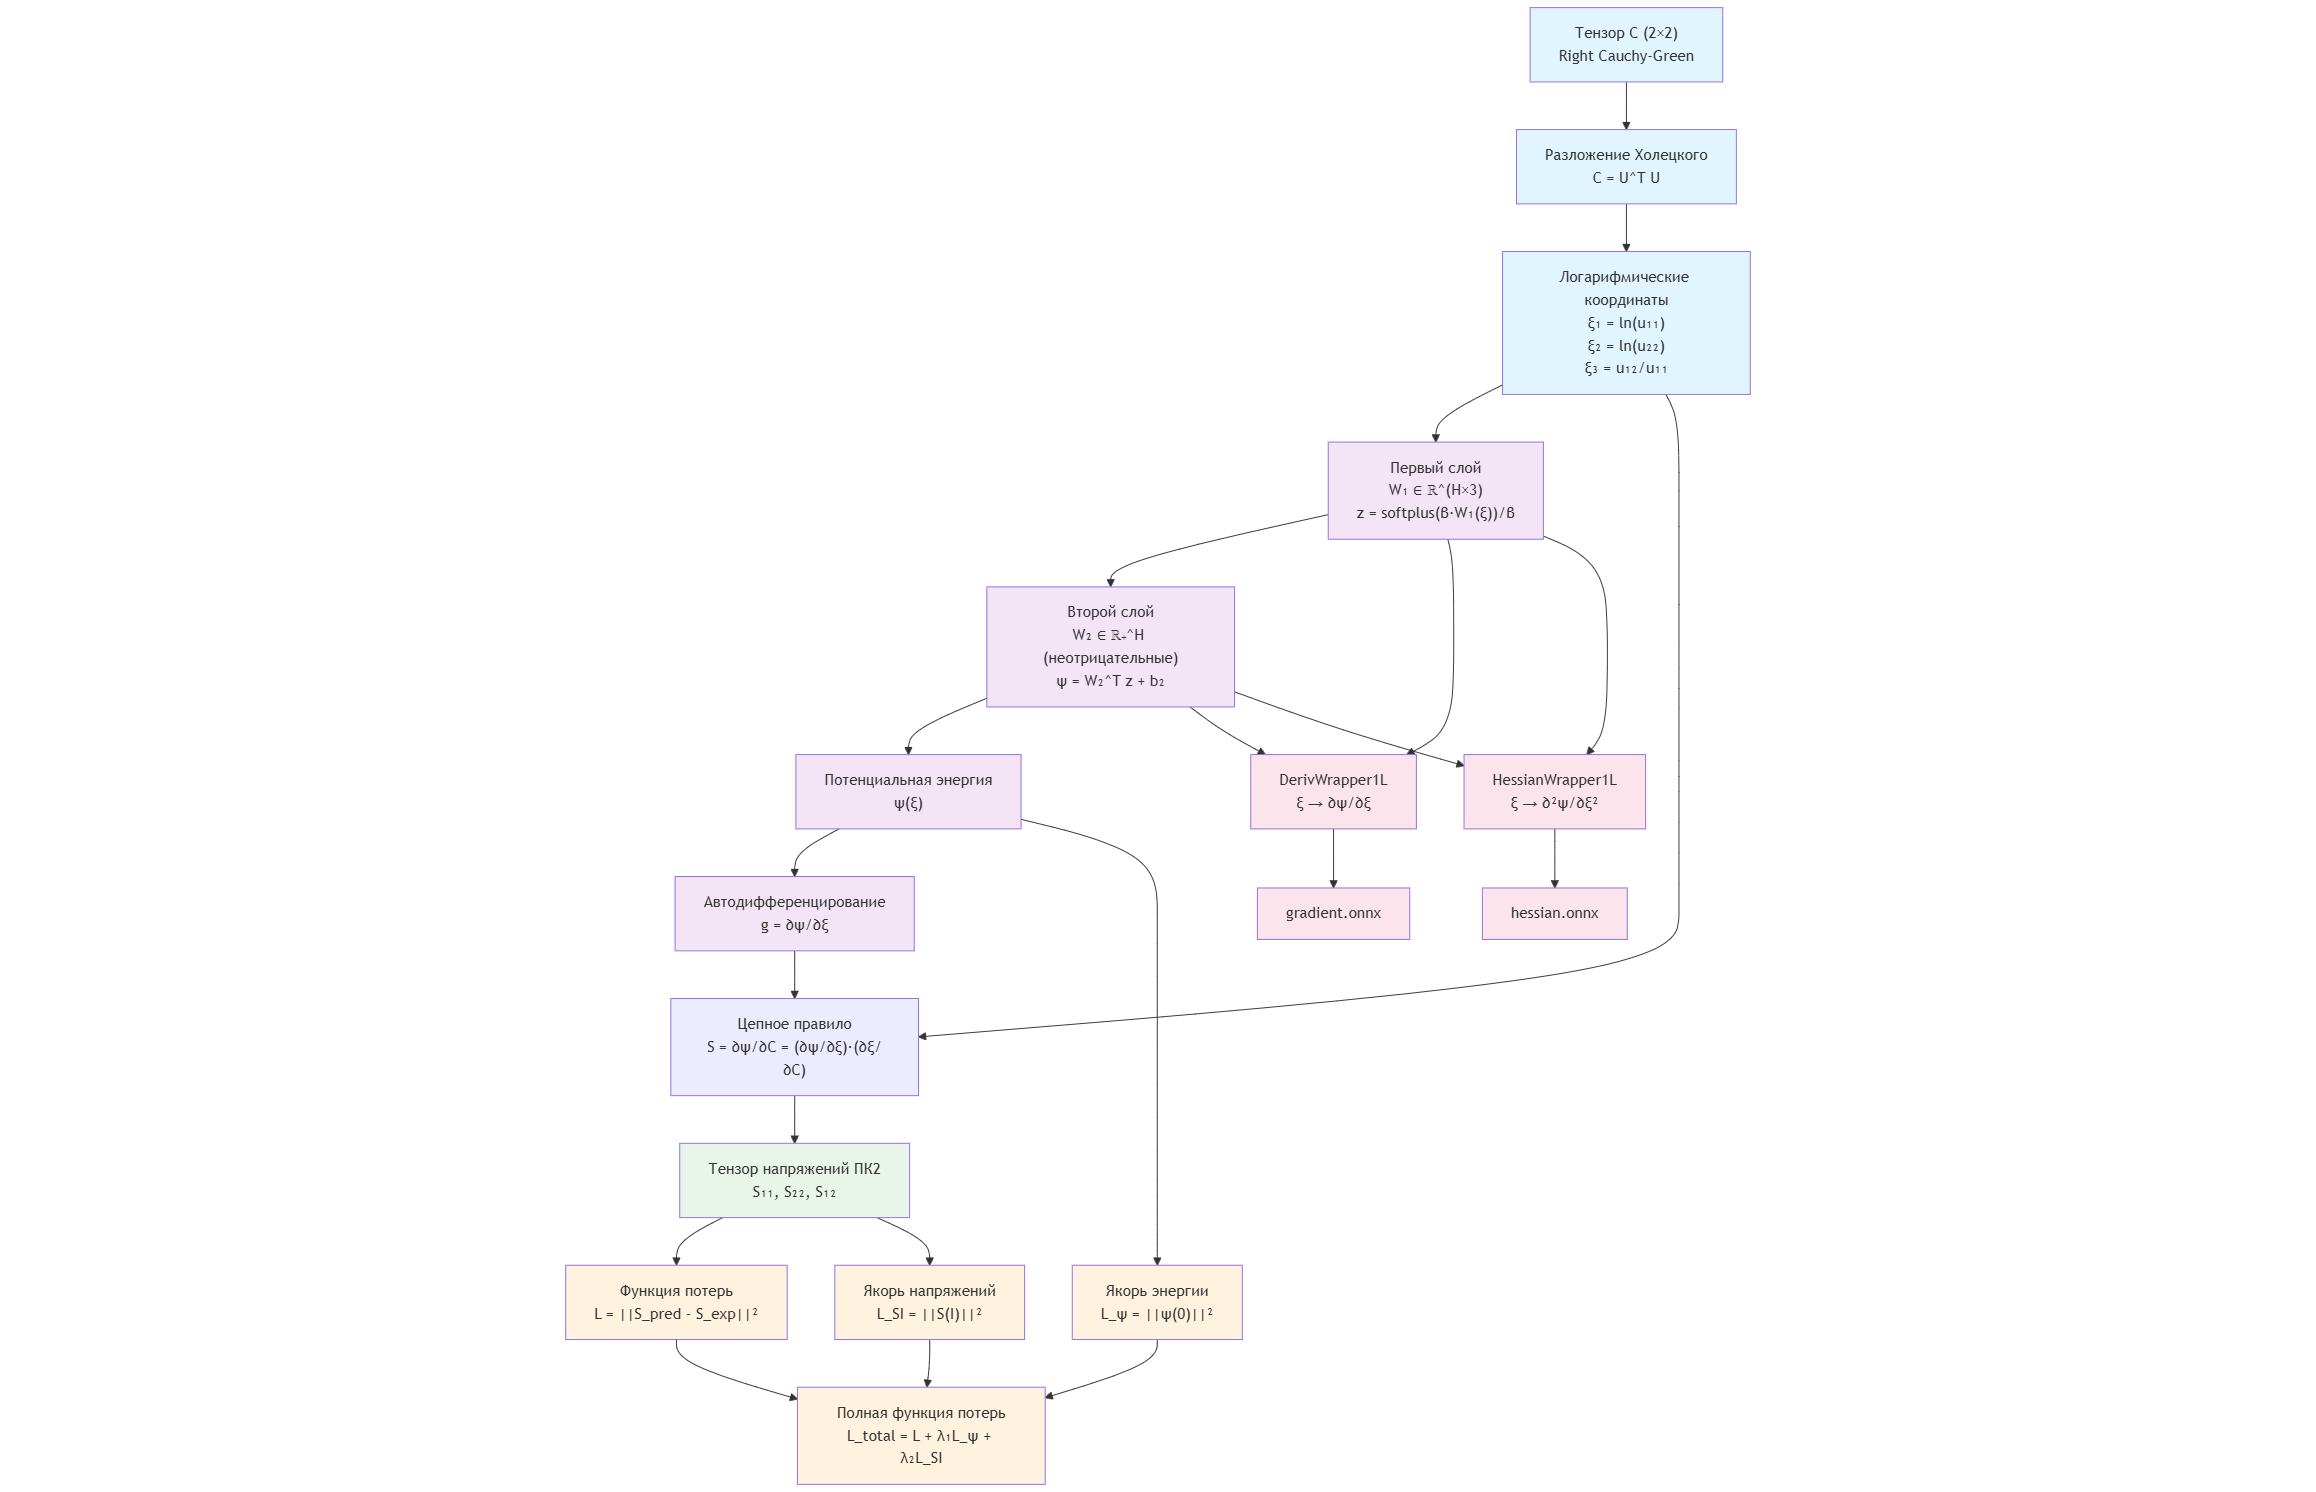
\includegraphics[width=1.3\textwidth]{img/clann_arc.png}
\caption{Схема вычислительного процесса CLANN: от входного тензора до функции потерь. Показаны этапы обработки входных данных, вычисления нейросетью, дифференцирования и формирования функции потерь.}
\label{fig:clann_architecture}
\end{figure}

\textbf{Аналитические выражения для производных энергии}

\textbf{Градиент энергии деформации}

Аналитическое дифференцирование функции энергии по переменным \(\xi\) даёт выражение для градиента:

\begin{equation}
 \nabla_\xi \psi = \vect W_1^T \left( \vect W_2 \odot \sigma(\beta (\vect W_1 \vect \xi + \vect b_1)) \right),
\label{eq:energy_gradient}
\end{equation}

где $\sigma(x) = \frac{1}{1 + e^{-x}}$ - сигмоида, 
а операция $\odot$ обозначает поэлементное произведение (Hadamard product). 
Данное выражение демонстрирует, что градиент энергии является линейной комбинацией строк матрицы $\vect W_1^T$ с весами, 
определяемыми произведением выходных весов $\vect W_2$ и значений функции активации $\sigma(\beta (\vect W_1 \vect\xi + \vect b_1))$.

\textbf{Гессиан энергии деформации}

Вторые производные энергии по переменным \(\xi\) определяют гессиан, который имеет следующую аналитическую форму:

\begin{equation}
 H_{ij} = \sum_h \sigma'_h\,W_{2,h}\,W_{h,i}W_{h,j},
\label{eq:energy_hessian}
\end{equation}

где $\sigma' = \beta\,\sigma(1-\sigma)$ - производная сигмоиды, 
$\sigma=\operatorname{sigmoid}(\beta s)$, а $s=\vect W_1\xi+\vect b_1$.

\textbf{Материальная устойчивость и положительная определённость}

% Строгая выпуклость функции энергии \(\psi(\xi)\) по переменным \(\xi\)
% имеет фундаментальное значение для материальной устойчивости гиперупругого материала. 
% Как показано в классических работах Болла (Ball, 1977) и Чиарлета (Ciarlet, 1988), 
% выпуклость энергии деформации является необходимым и достаточным условием для существования и единственности решения 
% задачи равновесия в нелинейной теории упругости.

Из строгой выпуклости \(\psi(\xi)\) следует положительная определённость гессиана:
\begin{equation}
 \vect H = \frac{\partial^2\psi}{\partial\xi^2} > 0,
\label{eq:positive_hessian}
\end{equation}

что обеспечивает положительную определённость касательных модулей упругости 
$\mathbb{C} = \partial^2\psi/\partial\vect C^2$ через цепное правило дифференцирования. 
Это свойство важно для численной стабильности конечно-элементных расчётов, 
поскольку на практике обеспечивает сходимость метода Ньютонаи отсутствие сингулярностей в матрице жёсткости.

% \textbf{Физическая интерпретация гессиана}

% Гессиан $H_{ij}$ представляет собой матрицу касательных модулей упругости в логарифмических координатах Лапласа. Положительная определённость этой матрицы, обеспечиваемая архитектурой ICNN, гарантирует материальную устойчивость в том смысле, что любое малое возмущение деформации приводит к увеличению энергии деформации. Это свойство является фундаментальным для гиперупругих материалов и соответствует принципу Ле Шателье-Брауна в термодинамике.

% Структура выражения \eqref{eq:energy_hessian} отражает аддитивный вклад каждого скрытого нейрона в общую жёсткость материала, что обеспечивает физически интерпретируемую параметризацию механических свойств.

% \subsection{Функция потерь и процесс обучения: физические ограничения и регуляризация}

% \textbf{Основная функция потерь: минимизация невязки напряжений}

В рамках предложенного подхода обучение модели осуществляется путём минимизации функции потерь, 
которая количественно характеризует невязку между предсказанными и экспериментальными значениями напряжений:

\begin{equation}
 L = \frac{1}{N}\sum_{i=1}^N \lVert \vect S^{(i)}_{\text{pred}} - \vect S^{(i)}_{\text{exp}} \rVert^2.
\label{eq:main_loss_function}
\end{equation}

% Данная функция потерь имеет глубокий физический смысл, поскольку минимизация невязки напряжений эквивалентна минимизации работы внешних сил на виртуальных перемещениях, что соответствует принципу виртуальных работ в механике сплошных сред.

% \textbf{Физические ограничения и регуляризация}

% Для обеспечения физической корректности модели в функцию потерь вводятся дополнительные слагаемые, 
% отражающие принципы механики:

% \begin{equation}
%  L_{\text{SI}} = \lVert \vect S(\vect I)\rVert^2,\qquad L_{\psi}=\lVert\psi(0)\rVert^2.
% \label{eq:physical_constraints}
% \end{equation}

% Первое слагаемое $L_{\text{SI}}$ обеспечивает выполнение условия естественного состояния: 
% при отсутствии деформации ($\vect C = \vect I$) тензор напряжений должен обращаться в нуль. 
% Это условие является прямым следствием принципа объективности и соответствует физическому требованию 
% отсутствия внутренних напряжений в недеформированном состоянии.

% Второе слагаемое $L_{\psi}$ гарантирует, что энергия деформации в естественном состоянии равна нулю.

% \textbf{Полная функция потерь и процесс оптимизации}

% Объединение основного функционала потерь с физическими ограничениями даёт полную функцию потерь:

% \begin{equation}
%  L_{\text{total}} = L + \lambda_{\text{SI}} L_{\text{SI}} + \lambda_{\psi} L_{\psi}.
% \label{eq:total_loss_function}
% \end{equation}

% Коэффициенты $\lambda_{\text{SI}}$ и $\lambda_{\psi}$ определяют относительную важность физических ограничений 
% по сравнению с точностью аппроксимации экспериментальных данных. 
% Их выбор является критически важным для баланса между точностью модели и физической корректностью.

Для минимизации функции потерь \eqref{eq:main_loss_function} используется оптимизатор Adam \cite{kingma2014adam}, 
который широко используется в задачах машинного обучения. 
Процесс оптимизации включает вычисление градиентов по всем параметрам сети и обновление весов 
с использованием адаптивных моментов первого и второго порядка.

Такое построение архитектуры CLaNN обеспечивает выполнение всех необходимых физических свойств гиперупругой модели: 
\textbf{термодинамическая корректность} достигается через строгое соблюдение соотношения \eqref{eq:chain-rule}, 
что гарантирует консервативность напряжений $\oint \vect{S}:\mathrm{d}\vect{C} = 0$ и согласованность с законами 
термодинамики; 
\textbf{материальная устойчивость} обеспечивается и существенно улучшается за счёт строгой выпуклости функции энергии 
$\psi(\boldsymbol{\xi})$, гарантируемой архитектурой ICNN ($\vect{W}_2 \ge 0$, выпуклая неубывающая активация); 
\textbf{объективность} автоматически выполняется благодаря параметризации через тензор 
Коши-Грина $\vect{C} = \vect{F}^{\top}\vect{F}$, обеспечивая инвариантность относительно поворотов и симметрию напряжений; 
\textbf{строгая неотрицательность и коэрцитивность энергии} обеспечиваются архитектурной калибровкой 
$\psi_{\mathrm{phys}}(\boldsymbol{\xi}) = \mathbf{W}_2^{\top}(z - z_0) - \mathbf{r}_0^{\top}\boldsymbol{\xi} + \tfrac{\gamma}{2}\|\boldsymbol{\xi}\|^2$ 
с $\gamma>0$, что даёт $\psi_{\mathrm{phys}}(\mathbf{0})=0$, $\psi_{\mathrm{phys}}(\boldsymbol{\xi})>0$ при $\boldsymbol{\xi}\ne\mathbf{0}$ и 
$\psi_{\mathrm{phys}}(\boldsymbol{\xi})\to\infty$ при $\|\boldsymbol{\xi}\|\to\infty$ (см. clann\_math.markdown, § Потенциал); 
\textbf{численная стабильность} достигается через логарифмическую параметризацию Лапласа \eqref{eq:laplace_coords}, которая корректно обрабатывает большие деформации и предотвращает нефизичные значения; 
наконец, \textbf{физические ограничения} \eqref{eq:energy_constraints} обеспечиваются архитектурой сети CLaNN: монотонные, выпуклые функции активации,
неотрицательные весовые коэффициенты, а также нормировка нулевого уровня энергии: из потенциальной энергии вычитается её значение в естественной конфигурации, что обеспечивает $\psi(0)=0$ и $\vect{S}(\vect{I})=\vect{0}$.



\section{Виртуальный эксперимент}

Мы используем синтетические экспериментальные данные для тестирования CLaNN 
на изотропном надуваним однородной и неоднородной по толщине мембраны. 
А именно, мы генерируем данные с помощью виртуальных экспериментов на плоских растяжениях образца и используем их в качестве входных данных для 
обучения CLaNN, без какого-либо дополнительного знания об изотропности/анизотропии образца и форме потенциала.
 
Обучение модели проводилось на численных экспериментальных данных, 
полученных при двухосном растяжении образца с геометрией мальтийского креста (Рисунок \ref{fig:malt_geometry}).
С неогуковской гиперупругой моделью для двумерной мембраны \cite{ogden1997nonlinear}
% \begin{equation}
%  \Psi(\vect C, T) = h_0\, \frac{\mu}{2}\,\big(\operatorname{tr}\vect C + T^2 - 3\big),
% \label{eq:neo_hookean_energy}
% \end{equation}
% где $\vect C$ — двумерный правый тензор деформаций Коши–Грина (вдоль срединной поверхности), $T$ — растяжение по толщине (параметр мембранного приближения), $h_0$ — начальная толщина мембраны, а $\mu = 0.432 \,\text{МПа}$ — модуль сдвига. Для несжимаемого материала выполняется связь $\sqrt{\det \vect C}\,T = 1$.

Причем данные для обучения собирались из одного центрального элемента сетки, что соответствует ограничениям эквивалетного 
натурного эксперимента, в котором невозможно установить без предположения модели материала полное поле напряжения в образце.

Для решения задачи равновесия гиперупругой мембраны используется метод описанный в \cite{ddaniso2024}.

\begin{figure}[H]
  \centering
  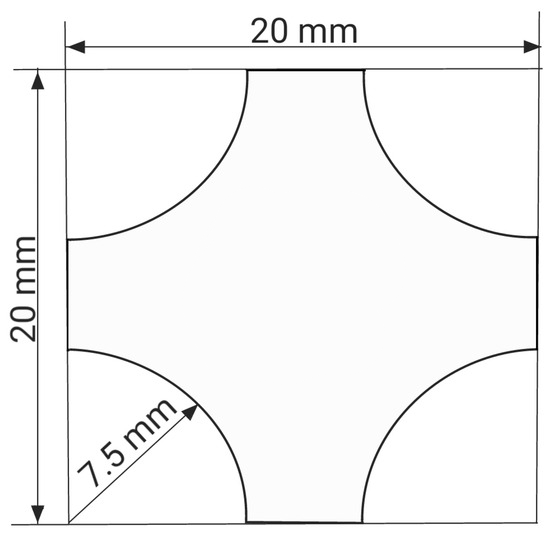
\includegraphics[width=0.5\textwidth]{img/malt_geom.png}
  \caption{Размеры образца биоматериала в форме мальтийского креста. 
  Радиус вырезов одинаков для всех вырезов}
  \label{fig:malt_geometry}
\end{figure}

Схематическое представление протоколов показано на рисунке \ref{fig:malt_displacements}, где $w_i \in [0,1]$, $i \in \{1,4\}$
представляет собой долю от заданного максимального смещения $u_{\max}$ для $i$-го плеча: $w_i = 0$ 
соответствует неподвижному плечу, а $w_i = 1$ — соответствует плечу, чьё положение было сдвинуто и фиксировано на расстояние $u_{max}$. 
Изменяя $w_i$, можно получить различные типы экспериментов. 
В наших виртуальных экспериментах мы постепенно 
прикладываем смещение с определенным шагом $\Delta s$ до достижения максимального смещения. 
Смещение $w_i \cdot n \cdot \Delta s$ прикладывается к $i$-му плечу на $n$-м шаге, где $n = 1, \ldots, N$, 
$N = u_{\max}/\Delta s$ — количество шагов. 
Треугольная сетка для образца является квазиравномерной с размером ячейки $h_{\text{fit}} = 0.25$ мм, максимальное смещение 
$u_{\max} = 2$ мм и $\Delta s = 0.2$ мм. 
На каждом шаге мы собираем данные $(\vect C, \vect S)$ для всех треугольников, принадлежащих центральной области. 
Поскольку мы используем линейные ($P_1$) конечные элементы, значения $(\vect C, \vect S)$ постоянны на каждом треугольнике.

 \begin{figure}[H]
  \centering
  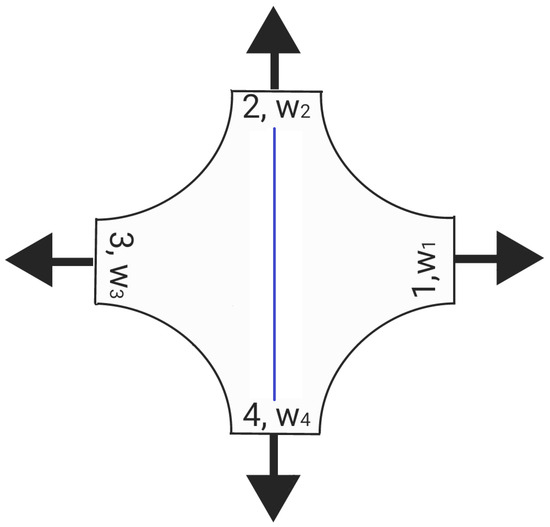
\includegraphics[width=0.5\textwidth]{img/malt_dirichlet.png}
  \caption{Схематическое представление протоколов. 
  Радиус вырезов одинаков для всех вырезов}
  \label{fig:malt_displacements}
\end{figure}
 
Наш предлагаемый тестовый протокол предполагает девять экспериментов:

\begin{table}[H]
\centering
\caption{Протоколы тестовых экспериментов}
\label{tab:test_protocols}
\begin{tabular}{|c|c|c|c|c|}
\hline
\textbf{№} & $w_1$ & $w_2$ & $w_3$ & $w_4$ \\
\hline
1 & 1 & 1 & 1 & 1 \\
2 & 1 & 0.75 & 1 & 0.75 \\
3 & 0.75 & 1 & 0.75 & 1 \\
4 & 1 & 0.5 & 1 & 0.5 \\
5 & 0.5 & 1 & 0.5 & 1 \\
6 & 1 & 1/3 & 1 & 1/3 \\
7 & 1/3 & 1 & 1/3 & 1 \\
8 & 1 & 0 & 1& 0 \\
9 & 0 & 1 & 0 & 1 \\
\hline
\end{tabular}
\end{table}

Обучающий набор содержал 90 точек данных правого тензора деформаций Коши-Грина $\vect C$ 
и второго тензора напряжений Пиолы-Кирхгофа $\vect S$.

\begin{figure}[H]
  \centering
  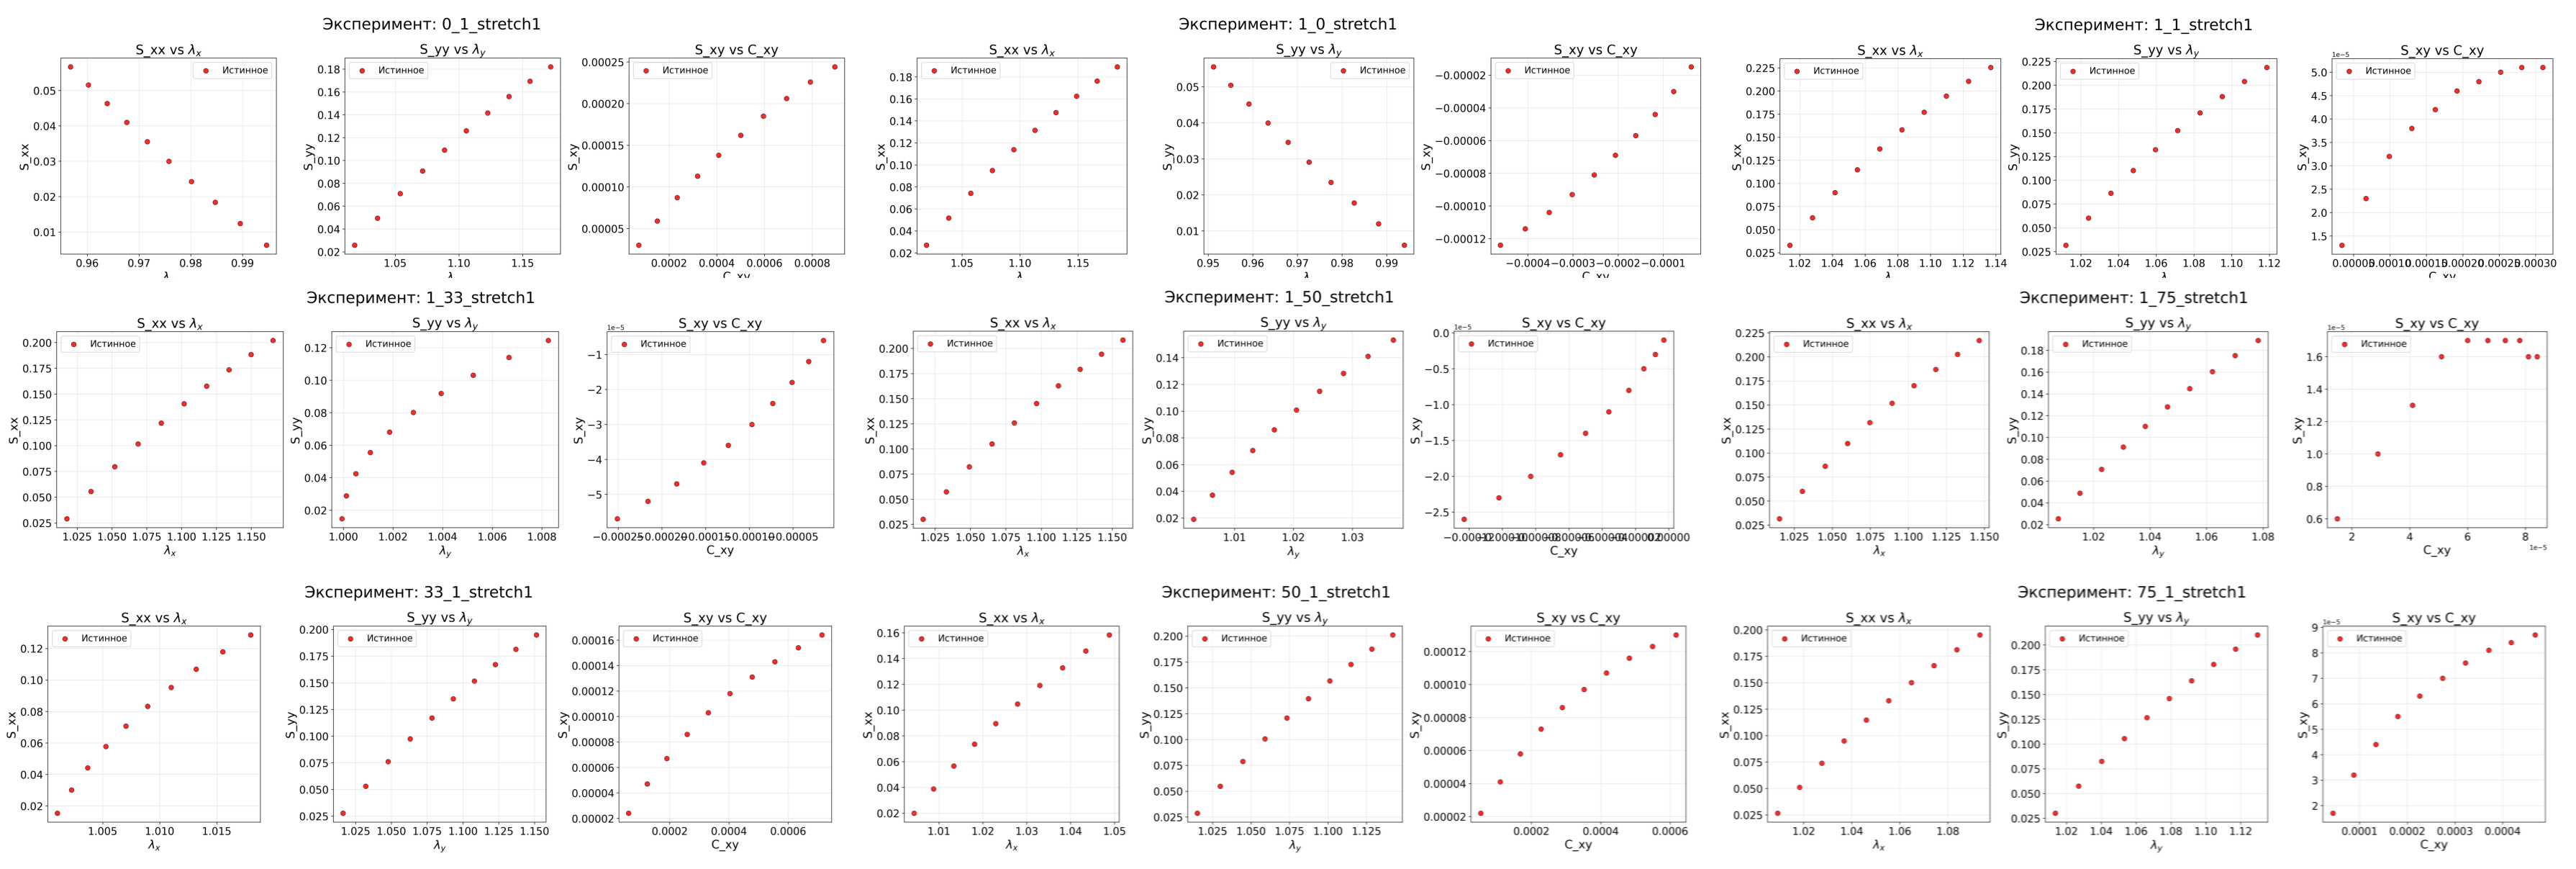
\includegraphics[width=1.0\textwidth]{img/all_stress_plots.png}
  \caption{Обучающий набор данных}
  \label{fig:training_data}
\end{figure}

\textbf{Гиперпараметры оптимизации:}
\begin{itemize}
  \item Скорость обучения (learning rate): $0.001$
  \item Размер батча (batch size): $128$
  % \item Веса физических ограничений: $\lambda_{\text{SI}} = 0.1$, $\lambda_{\psi} = 0.1$
  \item Архитектура: 16 нейронов на скрытом слое
\end{itemize}

\textbf{Результаты обучения:}
Процесс оптимизации показал высокую эффективность: ошибка аппроксимации снизилась на 5 порядков за менее чем 5000 эпох (рисунок \ref{fig:loss_curve}), 
что демонстрирует как качество предложенной архитектуры, так и корректность выбора функции потерь. 
Столь быстрая сходимость обусловлена строгой выпуклостью функции энергии, что обеспечивает единственность 
минимума и отсутствие локальных минимумов в пространстве параметров.

\begin{figure}[H]
  \centering
  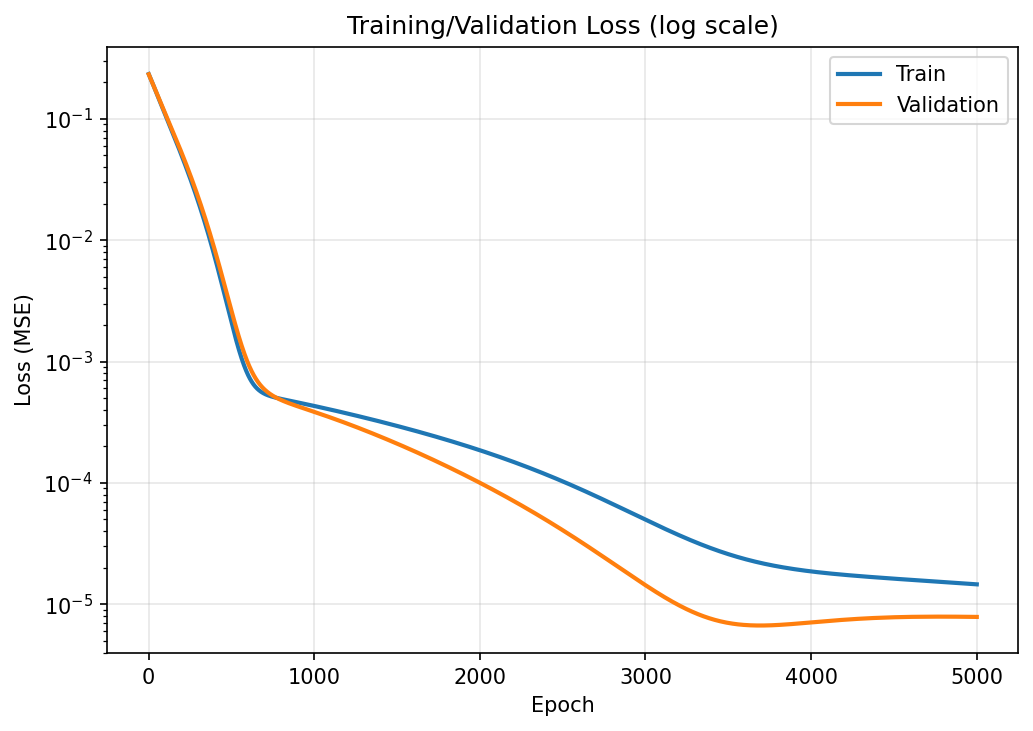
\includegraphics[width=0.7\textwidth]{img/loss_curve.png}
  \caption{Кривая функции потерь при обучении на 90 точках данных}
  \label{fig:loss_curve}
\end{figure}


\subsection{Интерполяция и экстраполяция кривых нагружения}
  Сначала мы проверили, как модель CLANN интерполирует и экстраполирует кривые нагружения.
  Для этого мы использовали 90 точек набора данных и разбивали его на различные соотношения обучающего и тестового наборов.
  Мы построили кривые нагружения на каждый протокол и сравнили их с экспериментальными данными.
  Для этого использовали коэффициент детерминации $R^2$, определяемый как:
  \begin{equation}
  R^2 = 1 - \frac{\sum_{i=1}^n (y_i - \hat{y}_i)^2}{\sum_{i=1}^n (y_i - \bar{y})^2},
  \label{eq:r_squared}
  \end{equation}
  где $y_i$ — экспериментальные значения, $\hat{y}_i$ — предсказания модели, $\bar{y}$ — среднее экспериментальных значений, $n$ — количество точек данных.
  Результаты представлены на рисунке \ref{fig:interpolation}.

  Для каждого протокола мы построили кривую нагружения и сравнили её с экспериментальными данными.
  
  \begin{figure}[H]
    \centering
    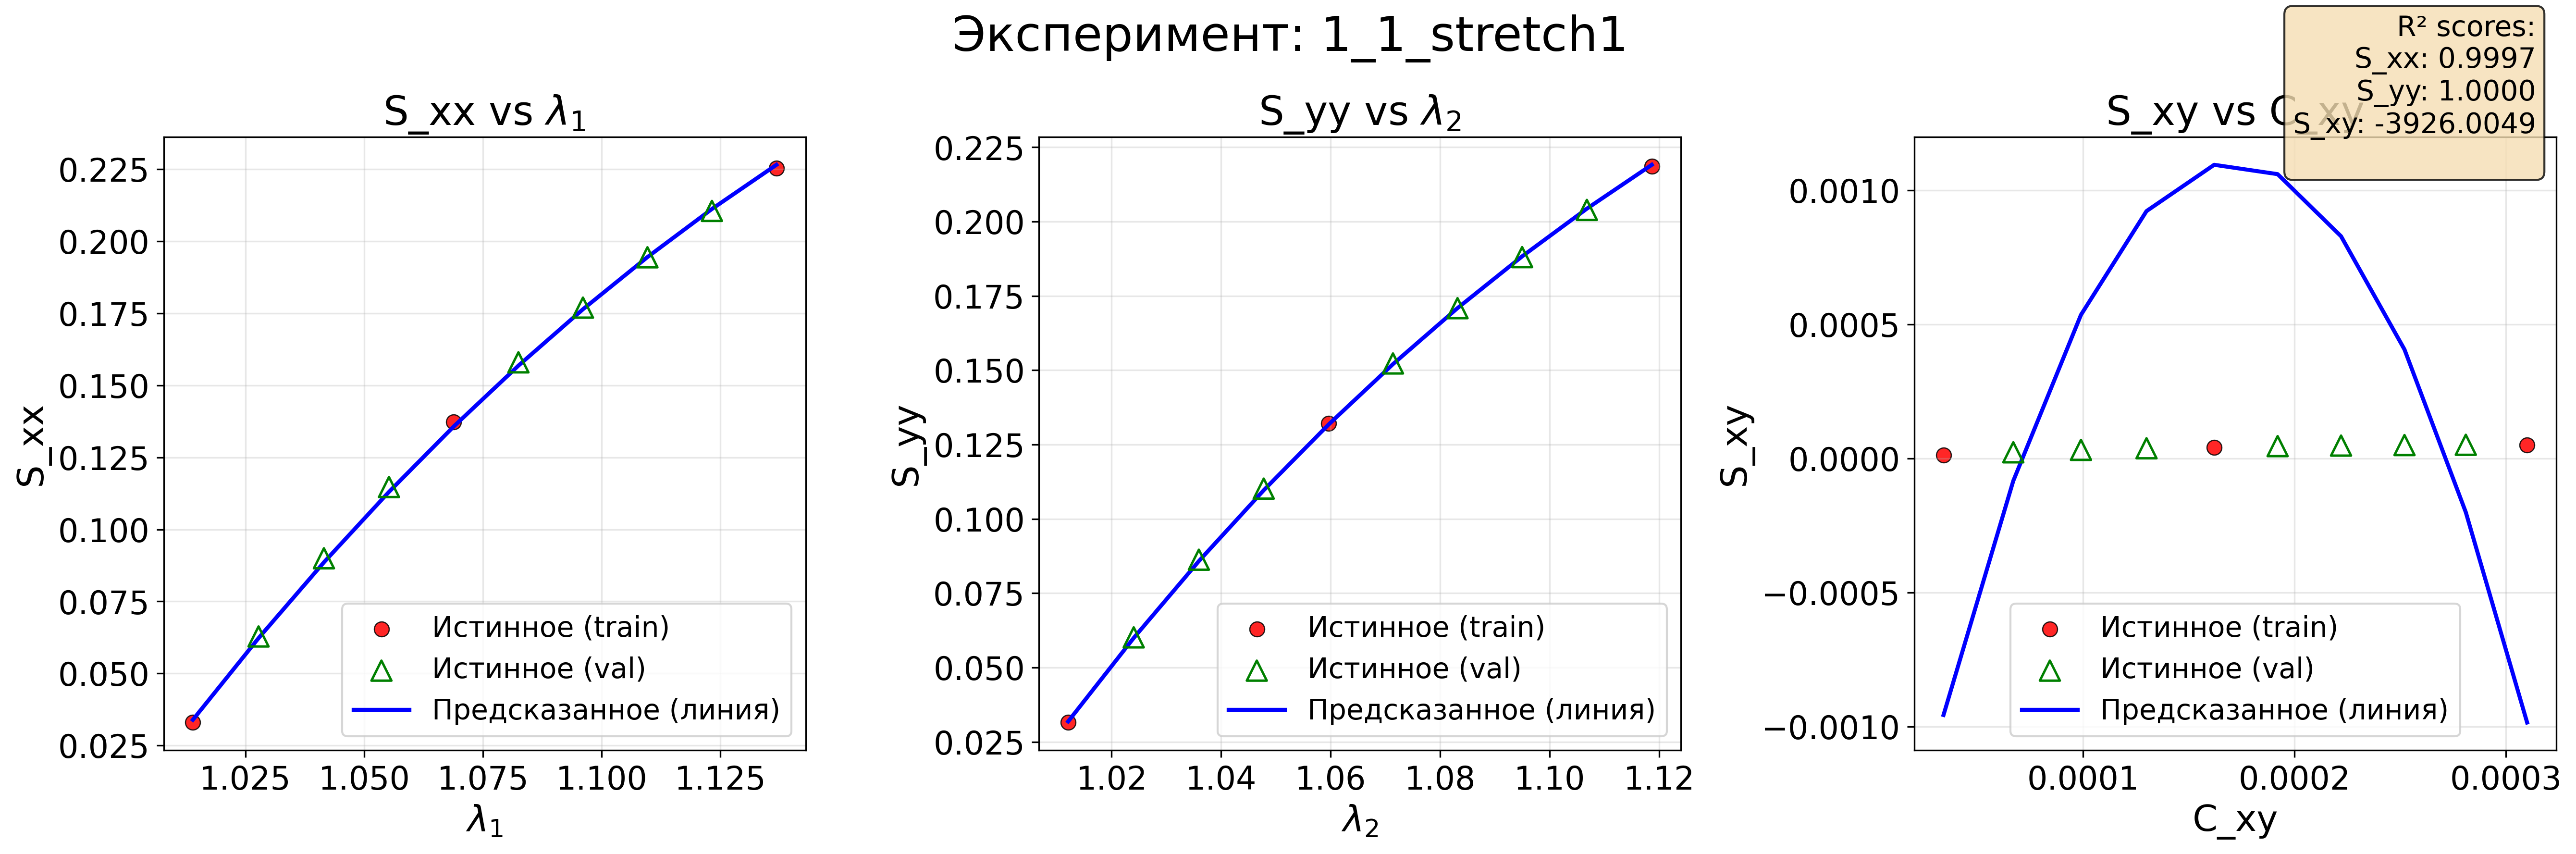
\includegraphics[width=1.0\textwidth]{img/interpolation.png}
    \caption{Кривая нагружения для равнодвухосного растяжения}
    \label{fig:interpolation}
  \end{figure}
  
  \begin{figure}[H]
    \centering
    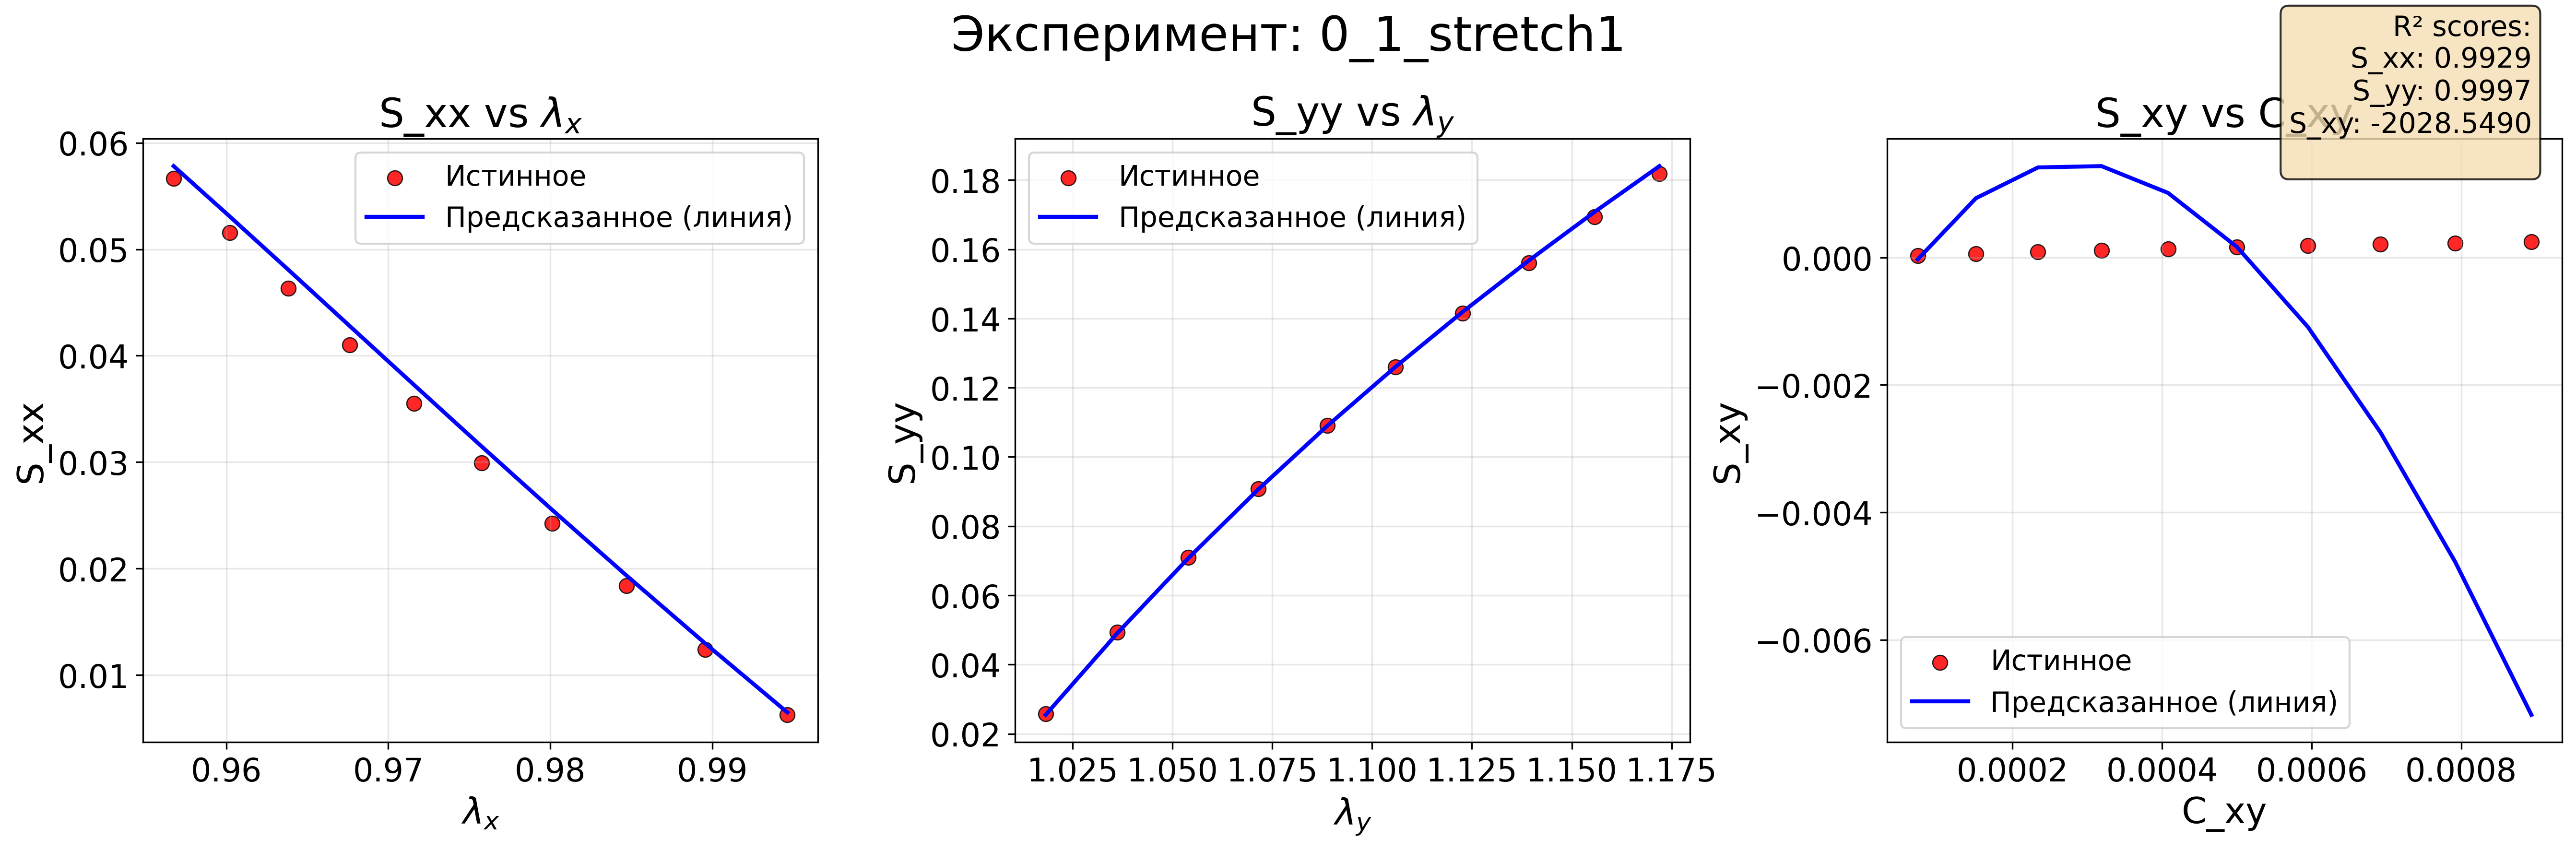
\includegraphics[width=1.0\textwidth]{img/extrapolation.png}
    \caption{Кривая нагружения для неравнодвухосного растяжения}
    \label{fig:extrapolation}
  \end{figure}
   
  

\subsection{Виртуальные эксперименты}

% \textbf{Разложение Холецкого и логарифмическая параметризация}

% Ключевым элементом предложенного подхода является использование разложения Холецкого для тензора правых деформаций Коши-Грина:

% \begin{equation}
% \vect C = \vect U^{\top}\vect U, \quad \vect U=\operatorname{cholesky\_upper}(\vect C).
% \label{eq:cholesky_decomposition}
% \end{equation}

% Данное разложение обеспечивает численную стабильность при больших деформациях, поскольку компоненты верхнетреугольного тензора $\vect U$ имеют ограниченные значения даже при значительных изменениях геометрии. Логарифмическая параметризация $\xi_i = \ln(u_{ii})$ дополнительно улучшает обусловленность задачи, что критически важно для численной устойчивости конечно-элементных расчётов.

% \textbf{Автоматическое дифференцирование и аналитические производные}

% В рамках предложенного подхода используется комбинированный подход к вычислению производных: автоматическое дифференцирование применяется для вычисления $\vect r=\partial\psi/\partial\xi$, в то время как аналитические формулы используются для определения напряжений $\vect S$ и гессиана $\vect H$. Такой подход обеспечивает оптимальный баланс между точностью вычислений и вычислительной эффективностью.

% Аналитические выражения для производных позволяют избежать дорогостоящих операций численного дифференцирования, что критически важно для интеграции в промышленные конечно-элементные пакеты. Кроме того, возможность экспорта вычислителей в онлайновые форматы (ONNX, TensorFlow) обеспечивает совместимость с широким спектром программного обеспечения для численного моделирования.

% \textbf{Интеграция в конечно-элементные расчёты}

% Интеграция предложенной модели в конечно-элементные расчёты осуществляется через стандартный интерфейс пользовательского материала (UMAT), где на каждом шаге итерации Ньютона требуются:

% \begin{enumerate}
%   \item Вычисление напряжений $\vect S$ для текущего состояния деформации
%   \item Определение касательных модулей упругости $\mathbb{C} = \partial^2\psi/\partial\vect C^2$
%   \item Обновление матрицы жёсткости элемента
% \end{enumerate}

% Положительная определённость гессиана $\vect H$ гарантирует положительную определённость матрицы жёсткости системы, что обеспечивает сходимость метода Ньютона и численную стабильность всего расчёта.

% \textbf{Физическая корректность и материальная устойчивость ICNN}

% Архитектура ICNN обеспечивает выполнение фундаментальных принципов механики сплошных сред, что делает предложенную модель физически корректной и численно стабильной.

% \textbf{Принцип объективности и инвариантность относительно поворотов}

% Модель инвариантна относительно произвольных поворотов системы координат благодаря параметризации энергии через инварианты деформации $\vect C$. Это свойство является прямым следствием принципа объективности, сформулированного Трусделлом (Truesdell, 1952), и гарантирует, что предсказания напряжений не зависят от выбора системы отсчёта. В терминах теории групп, данная инвариантность соответствует инвариантности относительно группы ортогональных преобразований $SO(3)$.

% \textbf{Материальная устойчивость через строгую выпуклость энергии}

% Строгая выпуклость функции энергии \(\psi(\xi)\) по переменным \(\xi\) обеспечивает выполнение условия материальной устойчивости в смысле Хаддамара (Hadamard, 1903). Это свойство гарантирует единственность решения задачи минимизации энергии и положительную определённость касательных модулей упругости, что критически важно для стабильности численного решения в конечно-элементных расчётах.

% \textbf{Положительность энергии деформации и термодинамическая корректность}

% Ограничение \(\vect W_2 \geq 0\) вместе с положительной активацией softplus гарантирует выполнение фундаментального принципа положительности энергии деформации, установленного ещё в работах Грина (Green, 1839). Это условие обеспечивает материальную устойчивость при больших деформациях и предотвращает нефизичные состояния с отрицательной энергией.

% \textbf{Численная стабильность и сходимость метода Ньютона}

% Положительная определённость гессиана \(\vect H = \partial^2\psi/\partial\xi^2\) обеспечивает сходимость метода Ньютона при решении нелинейных уравнений равновесия. Данное свойство особенно важно при больших деформациях, когда классические гиперупругие модели могут терять устойчивость вследствие потери положительной определённости касательных модулей упругости.

% \textbf{Регуляризация и обобщающая способность модели}

% Выпуклая структура ICNN естественным образом предотвращает переобучение и обеспечивает плавную интерполяцию между точками обучения. Модель демонстрирует способность к экстраполяции за пределы диапазона обучающих данных благодаря физически обоснованной структуре энергии, что является существенным преимуществом по сравнению с традиционными нейросетевыми подходами.

% \textbf{Вычислительная эффективность и аналитические производные}

% Аналитические выражения для градиента и гессиана позволяют избежать дорогостоящего численного дифференцирования, что критично для интеграции в промышленные конечно-элементные пакеты и расчётов в реальном времени. Данное свойство обеспечивает конкурентоспособность предложенного подхода с классическими гиперупругими моделями.

% \textbf{Термодинамическая согласованность и консервативность}

% Прямое вычисление напряжений из автоматического дифференцирования функции энергии по формуле \eqref{eq:hyperelastic_stress} гарантирует выполнение принципа консервативности напряжений, что является необходимым условием термодинамической корректности гиперупругой модели. Это свойство обеспечивает согласованность с первым законом термодинамики и принципом виртуальных работ.

% \section{Численные эксперименты и валидация модели}

% В рамках настоящего исследования проведён комплексный анализ предложенной модели CLANN посредством численных экспериментов, направленных на валидацию как физической корректности, так и численной эффективности подхода.

% \textbf{Эксперимент 1: Обучение на синтетических данных}

% Первоначальная валидация модели CLANN была проведена на синтетических данных, полученных при двухосном растяжении тела с геометрией мальтийского креста. В качестве эталонной модели использовался потенциал Нео-Гука, что позволило провести прямое сравнение с классическим подходом к гиперупругости. 

% \begin{table}[htbp]
% \centering
% \caption{Сводка проведенных экспериментов по обучению и валидации модели CLANN}
% \label{tab:experiments_summary}
% \begin{tabular}{|p{2.3cm}|p{2.2cm}|p{2.2cm}|p{1.3cm}|p{2.3cm}|p{1.5cm}|p{2.5cm}|}
% \hline
% \multicolumn{4}{|c|}{\textbf{Обучение}} & \multicolumn{3}{c|}{\textbf{Валидация}} \\
% \hline
% \textbf{Геометрия} & \textbf{Размер} & \textbf{Материал} & \textbf{Время} & \textbf{Геометрия} & \textbf{Время расчета} & \textbf{Количество элементов} \\
% \hline
% Мальтийский крест & 90 & Нео-Гук & -- & Гетерогенная круглая мембрана  & 329.816 сек & 4886 \\
% \hline
% Мальтийский крест & & & & Гомогенная круглая мембрана  & 329.816 сек & 4886  \\
% \hline
% Мальтийский крест & & & & Чистый сдвиг & -- сек & -- \\
% \hline
% \end{tabular}
% \end{table}

% \subsection{Сравнительный анализ с классическими гиперупругими моделями}

% Для всесторонней оценки качества и эффективности предложенной модели CLANN проведён детальный сравнительный анализ с классической гиперупругой моделью Нео-Гука. Данный выбор обусловлен тем, что модель Нео-Гука является фундаментальной в теории гиперупругости и широко используется как в теоретических исследованиях, так и в практических приложениях.

% \textbf{Теоретические основания для сравнения}

% Модель Нео-Гука характеризуется простейшей формой энергии деформации:
% \begin{equation}
% \psi_{\text{NH}} = \frac{\mu}{2}(I_1 - 3),
% \label{eq:neo_hooke_energy}
% \end{equation}

% где $\mu$ - модуль сдвига, а $I_1 = \text{tr}(\vect C)$ - первый инвариант тензора правых деформаций Коши-Грина. Данная модель обеспечивает линейную зависимость между девиаторными напряжениями и деформациями, что делает её идеальным кандидатом для валидации более сложных подходов.

% \textbf{Методология сравнительного анализа}

% Сравнительный анализ включал следующие аспекты:
% \begin{enumerate}
%   \item Точность аппроксимации экспериментальных данных
%   \item Численная стабильность при больших деформациях
%   \item Вычислительная эффективность
%   \item Способность к экстраполяции за пределы обучающего диапазона
% \end{enumerate}
% \textbf{Валидация на различных типах деформаций}

% Для всесторонней валидации модели CLANN на синтетических данных были проведены численные эксперименты с различными типами деформаций, включая одноосное растяжение, двухосное растяжение, чистый сдвиг и их комбинации. Данный подход позволил протестировать способность модели к описанию сложных деформационных состояний, характерных для реальных инженерных приложений.

% \textbf{Анализ численной устойчивости}

% Особое внимание было уделено анализу численной устойчивости предложенной модели при больших деформациях, где классические гиперупругие модели могут демонстрировать нестабильное поведение вследствие потери положительной определённости касательных модулей упругости. 

\begin{figure}[htbp]
\centering
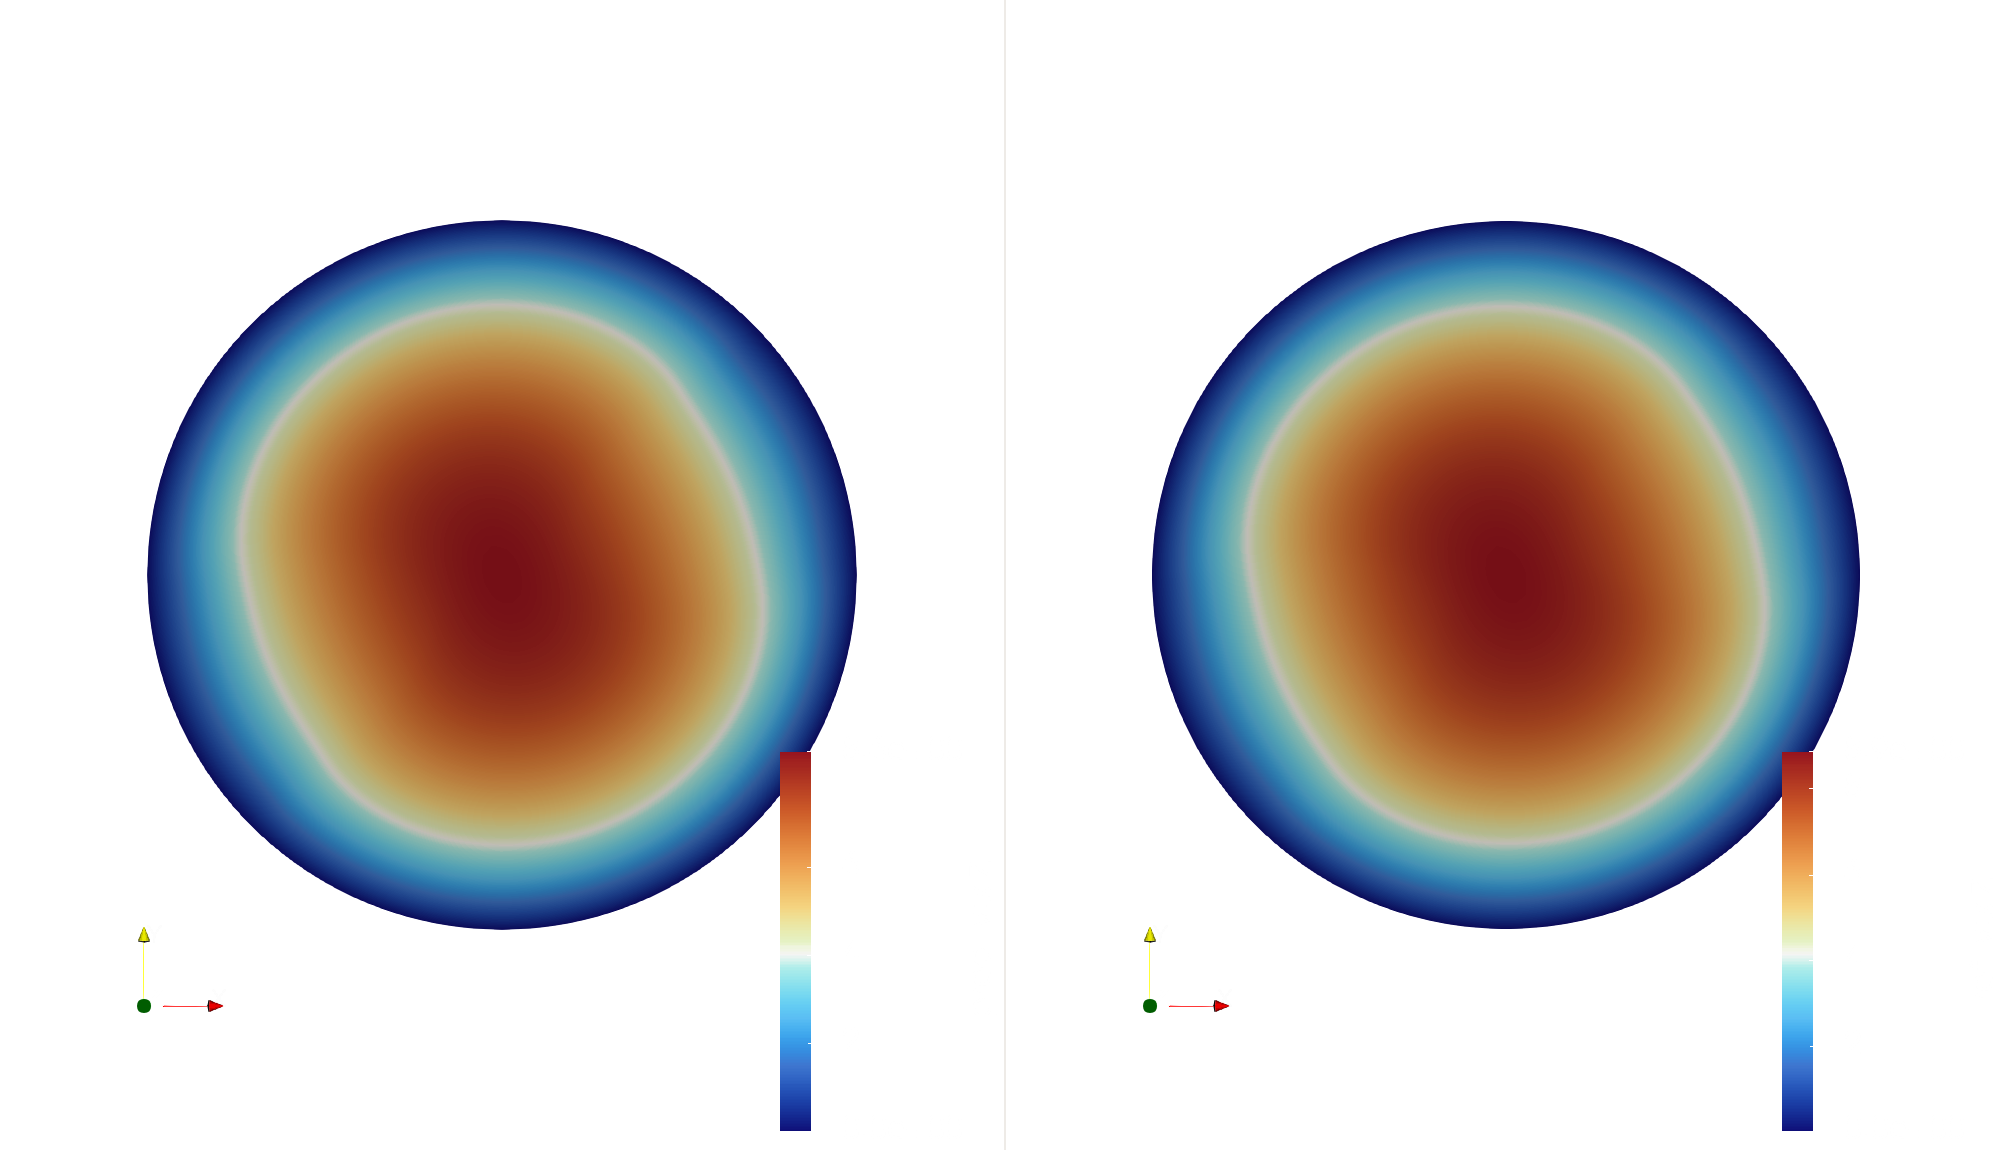
\includegraphics[width=0.8\textwidth]{img/bx_inf_u.png}
\caption{Результаты численного эксперимента: поле деформаций при различных типах нагружения. Показаны компоненты деформации $u_{11}$, $u_{22}$ и $u_{12}$ для различных конфигураций нагружения.}
\label{fig:numerical_deformations}
\end{figure}

\begin{figure}[htbp]
\centering
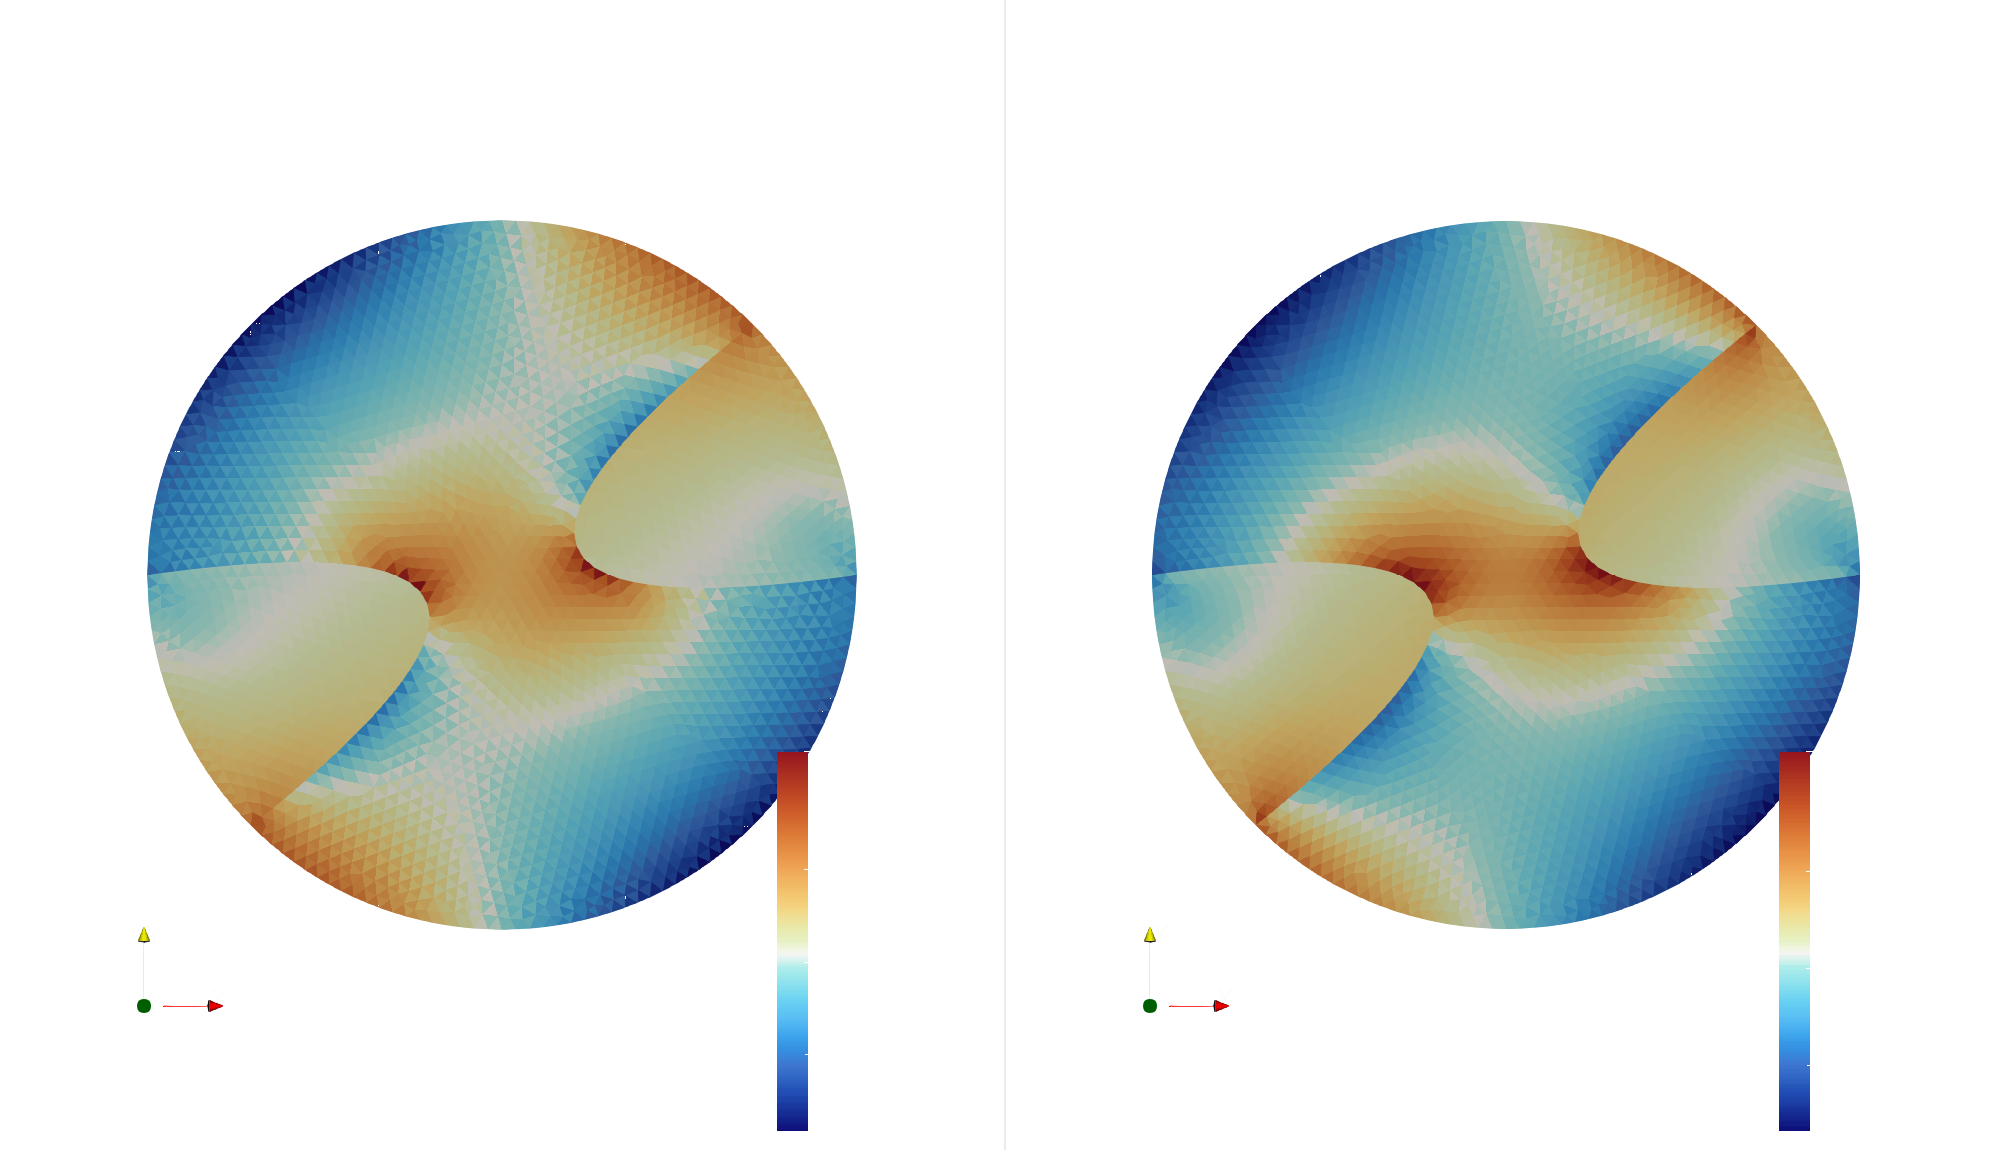
\includegraphics[width=0.8\textwidth]{img/bx_inf_S.png}
\caption{Результаты численного эксперимента: поле напряжений ПК2. Показаны компоненты напряжений $S_{11}$, $S_{22}$ и $S_{12}$, вычисленные моделью CLANN для соответствующих деформаций.}
\label{fig:numerical_stresses}
\end{figure}

\begin{figure}[htbp]
\centering
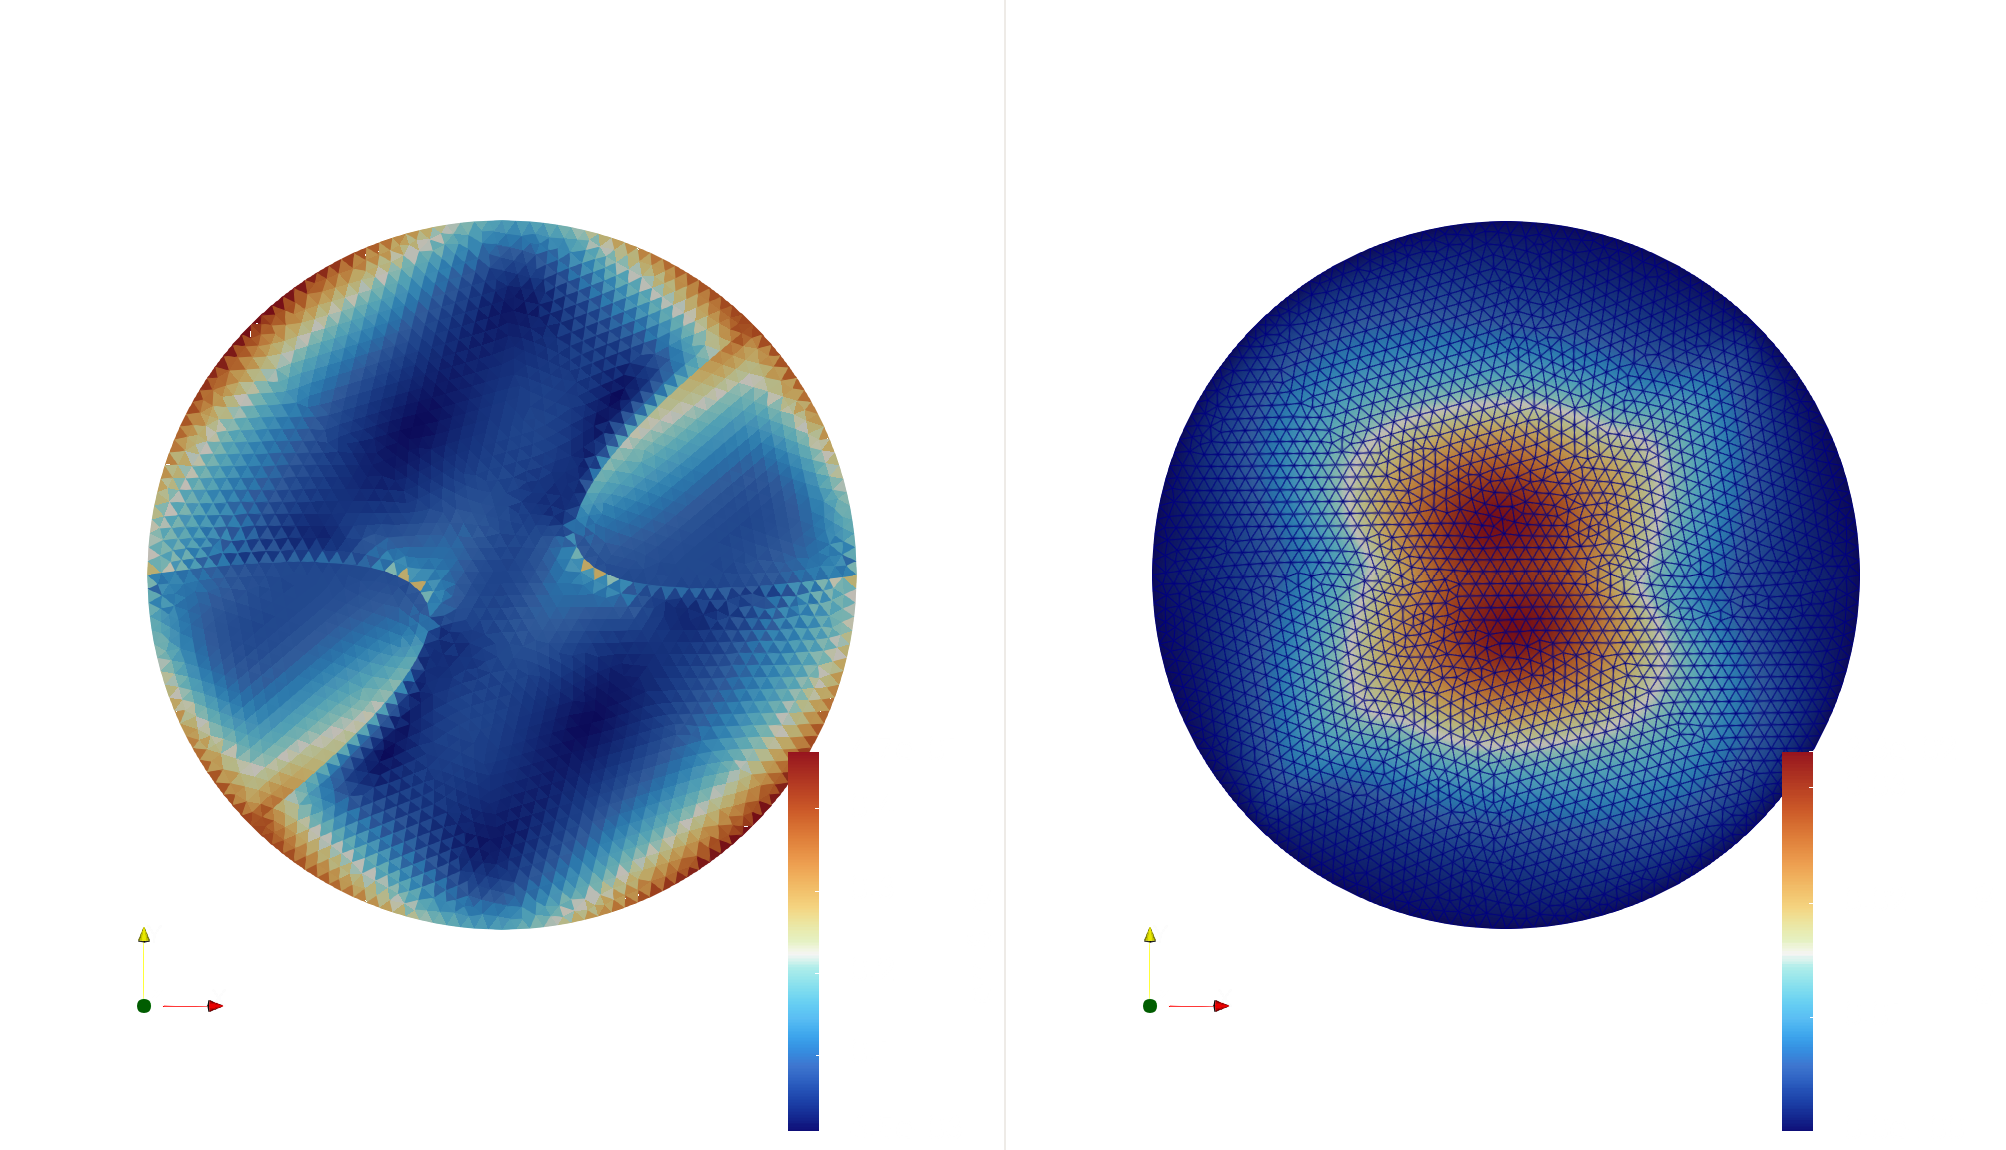
\includegraphics[width=0.8\textwidth]{img/bx_inf_err.png}
\caption{Анализ ошибок численного эксперимента: распределение относительных ошибок между предсказанными и эталонными значениями напряжений. Показаны локальные и глобальные метрики точности модели.}
\label{fig:numerical_errors}
\end{figure}


% \section{Натурные эксперименты}
% % Здесь будет содержание натурных экспериментов
% \subsection{Экспериментальная установка}
% % Описание экспериментальной установки

% \subsection{Результаты и валидация}
% % Результаты натурных экспериментов

\section{Заключение}
% Здесь будет заключение


% \section{Математические и термодинамические свойства}
% \subsection{Выпуклость и устойчивость}
% Строгая выпуклость \(\psi\) обеспечивает единственность минимума, положительную определённость касательной жёсткости и устойчивость численного решения.

% \subsection{Развёрнутый вывод через цепное правило и эквивалентные формы}
% Полная потенциальная энергия деформации задаётся композиционно
% \begin{equation}
%  \Psi(\vect C) = \psi\big(\xi(\vect C)\big),\quad \vect C = \vect F^{\top} \vect F,\quad \vect C = \vect U^{\top} \vect U,\ \xi = (\ln u_{11},\,\ln u_{22},\, u_{12}/u_{11}).
% \end{equation}
% Тензор ПК2 определяется как
% \begin{equation}
%  \vect S = \frac{\partial \Psi}{\partial \vect C}.
% \end{equation}
% Применяя цепное правило к \(\Psi(\vect C)\), получаем эквивалентную запись
% \begin{equation}
%  \frac{\partial \Psi}{\partial \vect C} = \frac{\partial \psi}{\partial \xi} : \frac{\partial \xi}{\partial \vect C} \equiv \vect g(\xi) : \vect J(\vect C),
% \end{equation}
% где \(\vect g(\xi)=\partial\psi/\partial\xi\in\mathbb{R}^3\) и \(\vect J(\vect C)=\partial\xi/\partial \vect C\) — тензор Якоби. В размерности 2D при выбранной параметризации и разложении Холецкого \(\vect C=\vect U^{\top} \vect U\) аналитическая подстановка даёт явные формулы для компонент \(\vect S\).

\appendix

\chapter{Эквивалентность QR-факторизации F и разложения Холецкого C=F$^{\top}$F для вычисления логарифмических координат $\boldsymbol{\xi}$}
\label{app:cholesky}

\section{Постановка и обозначения}

Рассматривается двумерная гиперупругая кинематика. Пусть:
\begin{itemize}
  \item $\vect F \in \mathbb{R}^{2 \times 2}$ — градиент деформации, $\det \vect F > 0$,
  \item $\vect C = \vect F^{\top}\vect F$ — правый тензор Коши–Грина (симметричный положительно определённый, SPD),
  \item Холецкий: $\vect C = \vect U^{\top}\vect U$, где $\vect U$ — верхнетреугольная и $\text{diag}(\vect U) > 0$,
  \item Логарифмические координаты:
    $\boldsymbol{\xi} = (\xi_1, \xi_2, \xi_3) = (\ln u_{11}, \ln u_{22}, u_{12}/u_{11})$.
\end{itemize}

Цель: показать, что при наличии $\vect F$ можно заменить вычисление $\vect U = \text{chol}(\vect C)$ на $\vect U = \vect R$ из тонкого QR($\vect F$) = $\vect Q \vect R$ (с $\text{diag}(\vect R) > 0$), и получить те же $\boldsymbol{\xi}$.

\section{Теорема (эквивалентность U и R)}

Пусть $\vect F \in \mathbb{R}^{2 \times 2}$ невырождённая ($\det \vect F > 0$). Рассмотрим тонкую QR-факторизацию
\begin{equation}
\vect F = \vect Q \vect R,
\end{equation}
где $\vect Q \in \mathbb{R}^{2 \times 2}$ — ортогональная ($\vect Q^{\top}\vect Q = \vect I$), $\vect R \in \mathbb{R}^{2 \times 2}$ — верхнетреугольная. Выберем стандартную нормализацию $\text{diag}(\vect R) > 0$. Тогда $\vect R$ совпадает с фактором Холецкого для $\vect C$:
\begin{equation}
\vect R = \text{chol}(\vect C), \quad \text{с} \quad \vect C = \vect F^{\top}\vect F.
\end{equation}

\textbf{Доказательство.}
\begin{equation}
\vect C = \vect F^{\top}\vect F = (\vect Q \vect R)^{\top}(\vect Q \vect R) = \vect R^{\top} \vect Q^{\top} \vect Q \vect R = \vect R^{\top} \vect R.
\end{equation}
Так как $\vect C$ — SPD и $\vect R$ — верхнетреугольная с положительной диагональю, то представление $\vect C = \vect R^{\top}\vect R$ единственно. По единственности фактора Холецкого (с $\text{diag} > 0$) следует $\vect R = \text{chol}(\vect C)$. $\square$

\textbf{Следствие.} Логарифмические координаты $\boldsymbol{\xi}$, определённые через $\vect U = \text{chol}(\vect C)$, можно эквивалентно вычислять из $\vect U = \vect R$ в QR($\vect F$), при условии $\text{diag}(\vect R) > 0$.

\section{Координаты $\vect{\xi}$ через $\vect{U}$}

Для $\vect U = \begin{bmatrix} u_{11} & u_{12} \\ 0 & u_{22} \end{bmatrix}$, $\text{diag}(\vect U) > 0$,
\begin{equation}
\boldsymbol{\xi} = (\xi_1, \xi_2, \xi_3) = (\ln u_{11}, \ln u_{22}, u_{12}/u_{11}).
\end{equation}
Тем самым, $\boldsymbol{\xi}(\vect F) := \boldsymbol{\xi}(\vect R(\vect F)) = \boldsymbol{\xi}(\vect U(\vect C))$.


